\documentclass[11pt,a4paper]{article}

%%% Packages %%%
\usepackage{amsmath,amsthm,amssymb,amsfonts}
\usepackage{mathrsfs}
\usepackage{tikz}
\usetikzlibrary{matrix,arrows,decorations.pathmorphing,positioning,calc}
\usepackage[colorlinks=true,linkcolor=blue,citecolor=blue,urlcolor=blue]{hyperref}
\usepackage{enumerate}
\usepackage{graphicx}
\usepackage{xcolor}

%%% Page geometry %%%
\usepackage[margin=1in]{geometry}

%%% Theorem environments %%%
\theoremstyle{plain}
\newtheorem{theorem}{Theorem}[section]
\newtheorem{proposition}[theorem]{Proposition}
\newtheorem{lemma}[theorem]{Lemma}
\newtheorem{corollary}[theorem]{Corollary}

\theoremstyle{definition}
\newtheorem{definition}[theorem]{Definition}
\newtheorem{example}[theorem]{Example}

\theoremstyle{remark}
\newtheorem{remark}[theorem]{Remark}

%%% Macros %%%
\newcommand{\C}{\mathbb{C}}
\newcommand{\Z}{\mathbb{Z}}
\newcommand{\N}{\mathbb{N}}
\newcommand{\Q}{\mathbb{Q}}
\newcommand{\R}{\mathbb{R}}
\newcommand{\GL}{\mathrm{GL}}
\newcommand{\gl}{\mathfrak{gl}}
\newcommand{\Sym}{\mathrm{Sym}}
\newcommand{\Rep}{\mathrm{Rep}}
\newcommand{\Crys}{\mathrm{Crys}}
\newcommand{\Vect}{\mathrm{Vect}}
\newcommand{\Set}{\mathrm{Set}}

%%% Title %%%
\title{Littlewood--Richardson Coefficients:\\
  From Puzzles to the Integrability Hierarchy}
\author{[To be determined]}
\date{April 2026}

\begin{document}

\maketitle

\begin{abstract}
% TODO: Write abstract.
%
% The abstract should cover:
% - LR coefficients as the central object (multiplicities in tensor products,
%   Schubert calculus, symmetric function structure constants)
% - The puzzle/honeycomb combinatorial perspective (Knutson--Tao--Woodward)
% - The integrable lattice model perspective (Zinn-Justin, Wheeler--Zinn-Justin)
% - The hierarchy: Yang--Baxter (braided) -> coboundary (cactus) -> crystal (symmetric)
%   as successive forgetting of structure
% - The categorical phase diagram organizing these levels
% - How every known combinatorial rule for LR coefficients fits into
%   this integrability hierarchy
%
Littlewood--Richardson coefficients $c_{\lambda\mu}^{\nu}$ govern the
multiplication of Schur functions, the decomposition of tensor products
of $\GL_n$ representations, and the intersection theory of Grassmannians.
We survey the landscape of combinatorial rules for these coefficients---from
the classical Littlewood--Richardson rule through Knutson--Tao--Woodward
puzzles to integrable lattice models---and organize them into a hierarchy
controlled by the Yang--Baxter equation and its degenerations.
At the top sits the fully solvable regime (braided monoidal, spectral parameter,
$R$-matrices); in the middle, the quasi-solvable or coboundary regime
(cactus group, crystals with commutor); at the bottom, the symmetric
monoidal regime (bare crystals, no spectral data). We argue that every
known combinatorial rule for $c_{\lambda\mu}^{\nu}$ and its
$K$-theoretic and equivariant generalizations finds a natural home in
this categorical phase diagram, and we identify the open problems that
remain.
% TODO: Revise and polish once all sections are complete.
\end{abstract}

\tableofcontents

\bigskip

%%% Section files %%%
%% Section 1: Introduction
%% Paper: Littlewood-Richardson Coefficients: From Puzzles to the Integrability Hierarchy

\section{Introduction}\label{sec:introduction}

The Littlewood-Richardson coefficients $c^\lambda_{\mu\nu}$ are among the most
studied numbers in algebraic combinatorics.  They appear as the structure
constants of the ring of symmetric functions,
\begin{equation}\label{eq:lr-def}
  s_\mu \cdot s_\nu \;=\; \sum_\lambda c^\lambda_{\mu\nu}\, s_\lambda,
\end{equation}
as tensor product multiplicities of $GL_n$ representations, and as intersection
numbers in the Schubert calculus of Grassmannians.  What is remarkable is not
that they can be computed---they can, in many ways---but that so many
\emph{independent} combinatorial interpretations coexist.  The
Littlewood-Richardson rule counts skew tableaux satisfying a lattice word
condition.  The Knutson-Tao-Woodward puzzle model~\cite{knutson-tao-woodward-2004}
tiles a triangle with three species of unit rhombi.  Purbhoo's
mosaics~\cite{purbhoo-2007} give a hybrid between the two.  Pipe dreams and
bumpless pipe dreams compute the same numbers via reduced decompositions in the
symmetric group.  Gaetz and Gao's interlacing triangular
arrays~\cite{gaetz-gao-2024} provide yet another model, discovered from
the geometry of Coxeter groups.  Each of these was found independently, often
by different communities---algebraists, combinatorialists, geometers---and the
bijections connecting them, while known, have the character of ad hoc
constructions.  One is left with a question that is more structural than
computational: \emph{why do all of these models exist?}

\subsection*{The integrable perspective}

The first hint of a deeper explanation came from Zinn-Justin's
observation~\cite{zinn-justin-2008} that KTW puzzle pieces \emph{are} the
Boltzmann weights of an exactly solvable lattice model.  More precisely, the
three puzzle tiles carry weights that satisfy the \emph{Yang-Baxter equation}
(YBE), the fundamental integrability condition for two-dimensional statistical
mechanics.  This is not a metaphor.  The row transfer matrix of the lattice
model literally processes the puzzle triangle row by row, and its partition
function evaluates to $c^\lambda_{\mu\nu}$.  The YBE guarantees that the
transfer matrices for different rows commute, which is why the boundary data
(the partitions $\lambda$, $\mu$, $\nu$) determine the count regardless of the
internal tiling---exactly as they should, since the LR coefficient depends on
the partitions alone.

Bump and Naprienko~\cite{bump-naprienko-2025} elevated this observation to a
structural principle.  They introduced the \emph{Yang-Baxter groupoid}: its
objects are combinatorial models (each specified by a choice of boundary
conditions and local vertex weights), and its morphisms are R-matrix
transformations arising from the YBE.  Two models connected by a morphism
compute the same structure constants.  Within this framework, the ``mysterious''
bijections between puzzles, tableaux, and pipe dreams become groupoid morphisms
---canonical consequences of the Yang-Baxter equation rather than feats of
combinatorial ingenuity.  At a still deeper level, Garbali and
Gunna~\cite{garbali-gunna-2024} showed that all vertex models in this story
are representations of the Feigin-Odesskii \emph{shuffle algebra}, providing a
single algebraic substrate from which the entire zoo of models can be derived.

\subsection*{The categorical phase diagram}

The Yang-Baxter groupoid explains the horizontal proliferation of models: many
combinatorial objects, all computing the same number, related by R-matrix moves.
But there is a second, orthogonal direction of variation that the groupoid alone
does not capture.  The LR coefficients are the \emph{classical} case---they
govern the cohomology ring of the Grassmannian.  One can deform to K-theory
(Grothendieck polynomials), to quantum K-theory, or to spin models
(Hall-Littlewood and $q$-Whittaker polynomials).  Each deformation has its own
integrable lattice model, its own R-matrix, and its own family of structure
constants---yet all satisfy the full Yang-Baxter
equation~\cite{wheeler-zinn-justin-2016, gunna-wheeler-zj-2025}.  The
deformation axis is orthogonal to the groupoid axis: it changes \emph{which}
structure constants are computed, not the mechanism by which models proliferate.

The central contribution of this paper is a \emph{categorical phase diagram}
that organises both directions simultaneously.  The horizontal axis parameterises
the deformation type (classical, K-theoretic, quantum K-theoretic, spin).  The
vertical axis parameterises the \emph{integrability level}---the categorical
structure that governs the symmetry of the model.  We identify three levels,
governed by the Hecke algebra chain $H_q \to H_0 \to \mathbb{C}[S_n]$:

\begin{enumerate}
\item \textbf{Braided monoidal} (generic $q$).  The Hecke generators satisfy
  $(T_i - q)(T_i + 1) = 0$, and the full Yang-Baxter equation holds.
  Symmetry is governed by the braid group $B_n$.  This is the world of
  Zinn-Justin's lattice models, Bump-Naprienko's groupoid, and the rich zoo
  of combinatorial models related by R-matrix moves.

\item \textbf{Coboundary monoidal} ($q = 0$).  At $q = 0$ the Hecke relation
  becomes $T_i(T_i + 1) = 0$; equivalently, the Demazure operators
  $\pi_i = T_i + 1$ satisfy $\pi_i^2 = \pi_i$, and the braiding
  degenerates.  What survives is a \emph{coboundary} structure: the commutor
  (the categorical analogue of the swap map) still exists, but it no longer
  satisfies the braid relation---only the weaker \emph{cactus group} relations
  of Henriques and Kamnitzer~\cite{henriques-kamnitzer-2006}.  This is the
  world of column-level integrability and the ``quasi-solvable'' models of
  Buciumas and Scrimshaw~\cite{buciumas-scrimshaw}.

\item \textbf{Symmetric monoidal} (crystal limit).  At the crystal level,
  $q$ is specialised away entirely, and only the symmetric group $S_n$ acts.
  The commutor becomes the trivial swap.  Crystal bases~\cite{kashiwara-1990}
  provide a purely combinatorial framework: Kashiwara operators, crystal graphs,
  tensor product rules.
\end{enumerate}

Each downward transition forgets something precise.  To state what, we recall
the \emph{Schur-Weyl decomposition}: for the defining representation $V$ of
$GL_n$, the tensor power decomposes as
\begin{equation}\label{eq:schur-weyl}
  V^{\otimes k} \;\cong\; \bigoplus_{\lambda \vdash k} V_\lambda \otimes S_\lambda,
\end{equation}
where $V_\lambda$ is the irreducible $GL_n$-module of highest weight $\lambda$
and $S_\lambda$ is the Specht module carrying the action of $S_k$.  The two
tensor factors---the ``physical'' space $V_\lambda$ and the ``multiplicity''
space $S_\lambda$---play sharply different roles in the hierarchy.

The key result (the \emph{Multiplicity Bundle Theorem}, proved in
Section~\ref{sec:hierarchy}) states that the coboundary commutor factorises as
\begin{equation}\label{eq:commutor}
  \sigma_{[i,j]} \;=\; \mathrm{id}_{V_\lambda} \otimes \rho_{S_\lambda}(w_0),
\end{equation}
where $w_0$ is the longest element of $S_{j-i+1}$ and $\rho_{S_\lambda}$
denotes the Specht module representation.  The commutor lives entirely in the
multiplicity space---it acts as the identity on the ``physical'' irreducible
$V_\lambda$ and as the longest-element involution on the Specht module
$S_\lambda$.  The crystal functor, which retains only the combinatorial skeleton
of the representation, kills the multiplicity space: since the tensor square
$B(\omega_1)^{\otimes 2}$ of the crystal of the defining representation is
multiplicity-free (a property special to the defining representation; the
general statement requires the Henriques-Kamnitzer crystal commutor theory),
every crystal automorphism is forced to be the identity by rigidity.  The
commutor becomes invisible.

This gives concrete mathematical content to each transition in the hierarchy.
The passage from braided to coboundary forgets the \emph{spectral parameter}:
the R-matrix $R(u)$, which depends on a continuous parameter $u$ and satisfies
the full parametric YBE, degenerates to the commutor $\sigma$, which is a
single fixed morphism satisfying only the cactus relations.  The passage from
coboundary to symmetric forgets the \emph{multiplicity bundle}: the Specht
module factor in~\eqref{eq:schur-weyl}, which carries the nontrivial action
of $\sigma$, is killed by the crystal functor, leaving only the symmetric
swap.

A crucial subtlety, clarified by Kamnitzer and
Tingley~\cite{kamnitzer-tingley-2007}: the coboundary structure is already
present at generic $q$, constructed from Drinfeld's unitarised R-matrix.
At $q = 0$, the braiding dies but the coboundary commutor survives.
The transition from braided to coboundary is not a creation but an
\emph{extraction}---the coboundary structure was always there, hidden inside
the braiding, and the $q = 0$ specialisation strips away the braided
superstructure to reveal it.  Like a zipper pulled open, the debraiding
separates two interlocking layers that were always distinct but moved in
concert.

\subsection*{Plan of the paper}

Section~\ref{sec:classical} reviews the classical theory of LR coefficients:
their definition via symmetric functions, tableaux, and Schubert calculus, and
the puzzle and Hopf algebra perspectives that set the stage for integrability.
Section~\ref{sec:lattice} introduces the integrable lattice model framework of
Zinn-Justin, presenting the Yang-Baxter equation and the transfer matrix
formalism.  Section~\ref{sec:groupoid} develops the Yang-Baxter groupoid of
Bump and Naprienko, explaining how classical bijections between combinatorial
models arise as groupoid morphisms.  Section~\ref{sec:hierarchy}, the heart of
the paper, constructs the categorical phase diagram and proves the Multiplicity
Bundle Theorem.  Section~\ref{sec:shuffle} briefly discusses the shuffle algebra
substrate underlying the entire framework.
Section~\ref{sec:open} collects open questions.

The picture that emerges is, we hope, both clarifying and aesthetically
satisfying.  The many combinatorial models for LR coefficients are not
historical accidents.  They are shadows of a single algebraic structure---the
integrable R-matrix and its degenerations---cast from different angles onto the
combinatorial plane.  The categorical phase diagram tells us which angles are
available, what is preserved at each level, and what is lost in each projection.
The coefficients themselves, those nonnegative integers governing the
multiplication of Schur functions, sit at the centre like a fixed point: the one
invariant that every shadow faithfully records.

%% Section 2: Classical Littlewood-Richardson Coefficients
%% To be \input{} into the main document.

\section{Classical Littlewood-Richardson Coefficients}
\label{sec:classical}

The Littlewood-Richardson coefficients $c^{\nu}_{\lambda,\mu}$ are
nonnegative integers that appear, independently and without apparent
conspiracy, in three different branches of mathematics.  That these
three appearances yield the \emph{same} number is already a theorem
worth contemplating.  We begin with the three definitions, then survey
the combinatorial models that make the coefficients computable, and
finally recast the entire story in the language of Hopf algebras and
transfer operators --- the doorway to integrability.

Throughout this section, our running example will be the coefficient
\[
  c^{(3,2,1)}_{(2,1),\,(2,1)} = 2.
\]
This is the smallest instance where the coefficient exceeds~$1$, and it
will accompany us into the lattice model of Section~3.

\subsection{Definitions and context}
\label{sec:classical-defn}

A \emph{partition} $\lambda = (\lambda_1 \ge \lambda_2 \ge \cdots \ge
\lambda_k > 0)$ is a weakly decreasing sequence of positive integers.
Its \emph{Young diagram} is the array of left-justified boxes with
$\lambda_i$ boxes in row~$i$; one may picture it as a skyline read
from left to right, each row a terrace one step narrower than the
last.  The \emph{size} $|\lambda| = \sum_i \lambda_i$ is the total
number of boxes.

\begin{definition}[LR coefficients: symmetric functions]
\label{def:lr-symm}
Let $\Lambda$ denote the ring of symmetric functions over $\mathbb{Z}$,
with its basis of Schur functions $\{s_\lambda\}$ indexed by partitions.
The \emph{Littlewood-Richardson coefficients} $c^{\nu}_{\lambda,\mu}$
are the structure constants of this basis:
\[
  s_\lambda \cdot s_\mu
  = \sum_{\nu} c^{\nu}_{\lambda,\mu}\, s_\nu.
\]
Since the Schur functions form a $\mathbb{Z}$-basis of $\Lambda$, the
coefficients are uniquely determined.  That they are
\emph{nonneg\-ative} is a deep fact, not at all obvious from this
definition.
\end{definition}

\begin{definition}[LR coefficients: representation theory]
\label{def:lr-rep}
Let $V_\lambda$ denote the irreducible polynomial representation of
$GL_n(\mathbb{C})$ of highest weight $\lambda$ (equivalently, the
Schur module associated to $\lambda$).  Then
\[
  V_\lambda \otimes V_\mu
  \cong \bigoplus_{\nu} V_\nu^{\oplus\, c^{\nu}_{\lambda,\mu}}
\]
as $GL_n$-representations.  Here the nonnegativity of the
coefficients is manifest: $c^{\nu}_{\lambda,\mu}$ is the multiplicity
of the irreducible $V_\nu$ in a tensor product, hence a dimension,
hence a nonneg\-ative integer.
\end{definition}

\begin{definition}[LR coefficients: Schubert calculus]
\label{def:lr-schub}
Let $\mathrm{Gr}(k,n)$ denote the Grassmannian of $k$-planes in
$\mathbb{C}^n$, and let $\sigma_\lambda \in H^*(\mathrm{Gr}(k,n))$
denote the Schubert class associated to a partition $\lambda$ fitting
inside a $k \times (n-k)$ box.  Then
\[
  \sigma_\lambda \cdot \sigma_\mu
  = \sum_\nu c^{\nu}_{\lambda,\mu}\, \sigma_\nu
  \quad \text{in } H^*(\mathrm{Gr}(k,n)).
\]
The geometric content: $c^{\nu}_{\lambda,\mu}$ counts the number of
points in a triple intersection of Schubert varieties in general
position.  Nonnegativity is again manifest --- one is counting
points.
\end{definition}

\begin{remark}
The fact that Definitions~\ref{def:lr-symm},~\ref{def:lr-rep},
and~\ref{def:lr-schub} give the same numbers is a consequence of the
Borel-Weil theorem and the classical relationship between the
representation ring of $GL_n$ and the cohomology of Grassmannians
(see \cite{fulton-1997} for a unified treatment).  But the
\emph{feeling} of the three definitions is quite different: in
$\Lambda$ the coefficients are algebraic, in representation theory
they are multiplicities, and in Schubert calculus they are
enumerative-geometric.  That a single integer can simultaneously be
all three things is what makes the LR coefficient a meeting place for
different parts of mathematics.
\end{remark}

The coefficients enjoy several structural properties that constrain
and enrich their study:

\begin{itemize}
\item \textbf{Symmetry.}
$c^{\nu}_{\lambda,\mu} = c^{\nu}_{\mu,\lambda}$, since multiplication
in $\Lambda$ is commutative.

\item \textbf{Vanishing.}
$c^{\nu}_{\lambda,\mu} = 0$ unless $|\nu| = |\lambda| + |\mu|$ and
$\nu \supseteq \lambda$, $\nu \supseteq \mu$ (containment of Young
diagrams).

\item \textbf{Saturation} (Knutson-Tao \cite{knutson-tao-1999}).
$c^{N\nu}_{N\lambda,\, N\mu} > 0$ if and only if
$c^{\nu}_{\lambda,\mu} > 0$.  In other words, the \emph{support} of
the LR coefficients is a saturated cone.  This resolved the
longstanding saturation conjecture and plays a key role in the Horn
inequalities characterizing eigenvalues of sums of Hermitian matrices.
\end{itemize}


\subsection{Combinatorial models}
\label{sec:classical-models}

The nonnegativity of $c^{\nu}_{\lambda,\mu}$ cries out for a
combinatorial proof: exhibit a set whose cardinality is
$c^{\nu}_{\lambda,\mu}$.  In fact, several such sets are known, each
illuminating a different aspect of the coefficient.

\subsubsection*{Skew tableaux and the Littlewood-Richardson rule}

Given partitions $\lambda \subseteq \nu$ (meaning $\lambda_i \le
\nu_i$ for all $i$), the \emph{skew shape} $\nu/\lambda$ is the set
of boxes in $\nu$ but not in $\lambda$ --- a diagram with a notch cut
from its northwest corner.

\begin{definition}[Semistandard Young tableau]
A \emph{semistandard Young tableau} (SSYT) of shape $\nu/\lambda$ and
\emph{content} $\mu = (\mu_1, \mu_2, \ldots)$ is a filling of the
boxes of $\nu/\lambda$ with positive integers such that:
\begin{enumerate}
\item[(i)] entries weakly increase along each row (left to right),
\item[(ii)] entries strictly increase down each column,
\item[(iii)] the number of entries equal to $i$ is $\mu_i$, for each $i$.
\end{enumerate}
\end{definition}

\begin{definition}[Lattice word]
The \emph{reverse reading word} of a tableau $T$ is obtained by
reading the entries of $T$ from right to left in each row, starting
from the top row.  A word $w_1 w_2 \cdots w_N$ is a \emph{lattice
word} (or \emph{ballot sequence}) if, for every prefix $w_1 \cdots
w_j$ and every letter $i$, the number of occurrences of $i$ in the
prefix is at least the number of occurrences of $i+1$.
\end{definition}

\begin{theorem}[Littlewood-Richardson rule; see {\cite[Ch.~5]{fulton-1997}}, {\cite[Ch.~7]{stanley-1999}}]
\label{thm:lr-rule}
The coefficient $c^{\nu}_{\lambda,\mu}$ equals the number of
semistandard Young tableaux of skew shape $\nu/\lambda$, content
$\mu$, whose reverse reading word is a lattice word.  Such tableaux
are called \emph{LR tableaux}.
\end{theorem}

\begin{example}[The coefficient $c^{(3,2,1)}_{(2,1),\,(2,1)} = 2$]
\label{ex:lr-tableaux}
The skew shape $(3,2,1)/(2,1)$ consists of three boxes: position
$(1,3)$ in the first row, position $(2,2)$ in the second row, and
position $(3,1)$ in the third row.  We seek fillings with content
$(2,1)$ --- two $1$s and one $2$ --- satisfying the semistandard and
lattice word conditions.

The two LR tableaux are:
\[
\young(\hfil\hfil1,\hfil1,2)
\qquad\text{and}\qquad
\young(\hfil\hfil1,\hfil2,1)
\]
where $\hfil$ denotes a box belonging to $\lambda = (2,1)$ (shaded or
omitted in the skew diagram).  In the first tableau the reverse
reading word is $1,1,2$ and in the second it is $1,2,1$; both are
lattice words.  The filling $\young(\hfil\hfil2,\hfil1,1)$ with
reverse reading word $2,1,1$ is \emph{not} a lattice word (the prefix
$2$ has more $2$s than $1$s), so it is excluded.  Hence
$c^{(3,2,1)}_{(2,1),(2,1)} = 2$.
\end{example}

\subsubsection*{Knutson-Tao-Woodward puzzles}

An entirely different model for the same coefficient was introduced by
Knutson, Tao, and Woodward \cite{knutson-tao-woodward-2004}.

\begin{definition}[KTW puzzle]
Fix a positive integer $N$.  An \emph{$N$-puzzle} is a tiling of an
equilateral triangle of side length $N$ by the following unit pieces,
each carrying labels $0$ or $1$ on its edges:
\begin{enumerate}
\item A triangle of side $1$ with all three edges labeled $0$.
\item A triangle of side $1$ with all three edges labeled $1$.
\item A \emph{rhombus} (two unit triangles glued along a shared edge)
with edges labeled $0$ and $1$ in the pattern: the two edges adjacent
to one acute angle are labeled $1$, and the two edges adjacent to the
other acute angle are labeled $0$.
\end{enumerate}
The three rhombus orientations (at $0^\circ$, $60^\circ$, and
$120^\circ$) are all permitted.  In a valid tiling, adjacent pieces
must agree on shared edges.

The boundary of the triangle consists of $3N$ edges, which we read as
three binary strings of length~$N$: the \textbf{south} side (left to
right), the \textbf{northeast} side (bottom to top), and the
\textbf{northwest} side (top to bottom).  A partition $\lambda$
fitting inside a $k \times (N-k)$ box is encoded as a binary string
of length $N$ via the boundary-path encoding described in
Section~\ref{sec:classical-hopf} below.
\end{definition}

\begin{theorem}[{\cite{knutson-tao-woodward-2004}}]
\label{thm:ktw}
For partitions $\lambda, \mu, \nu$ fitting inside a $k \times (N-k)$
box, the LR coefficient $c^{\nu}_{\lambda,\mu}$ equals the number of
$N$-puzzles whose south boundary encodes $\nu$, northwest boundary
encodes $\lambda$, and northeast boundary encodes $\mu$.
\end{theorem}

Each valid tiling is a \emph{puzzle witness}: a self-contained
combinatorial proof that one unit of $c^{\nu}_{\lambda,\mu}$ exists.
For our running example, the two tableaux of
Example~\ref{ex:lr-tableaux} correspond to two puzzle tilings of a
triangle of side $N=5$.  We will see in Section~3 that each tiling is
a \emph{configuration} of an integrable lattice model --- a
frozen-in-place snapshot of particle worldlines threading through the
triangle.

\begin{remark}
Purbhoo \cite{purbhoo-2007} established a direct bijection between
KTW puzzles and LR tableaux via an intermediate object called a
\emph{mosaic}, making the equivalence of Theorems~\ref{thm:lr-rule}
and~\ref{thm:ktw} constructive rather than merely numerical.
\end{remark}

The multiplicity of models is the paper's motivating mystery.  Why
should rhombus tilings (a geometric object), lattice-word conditions
on skew tableaux (a combinatorial object), and tensor product
multiplicities (a representation-theoretic object) all count the same
thing?  One answer --- the one this paper develops --- is that all
three are shadows of a single algebraic structure: an exactly solvable
lattice model whose transfer matrices commute by the Yang-Baxter
equation.

\subsection{The Hopf algebra perspective}
\label{sec:classical-hopf}

The three definitions of Section~\ref{sec:classical-defn} present LR
coefficients as \emph{structure constants} of a product.  But the ring
of symmetric functions carries more structure: it is a
\emph{self-dual graded connected Hopf algebra}, and the LR
coefficients appear equally in the coproduct.  This dual perspective
is less standard in the combinatorics literature, but it is the
natural home for transfer operators and the gateway to integrability.

\subsubsection*{The coproduct}

The ring $\Lambda$ of symmetric functions carries a coproduct
\[
  \Delta \colon \Lambda \to \Lambda \otimes \Lambda
\]
defined on the power-sum generators by $\Delta(p_k) = p_k \otimes 1 +
1 \otimes p_k$ and extended as an algebra homomorphism.  On the Schur
basis, the coproduct takes the form
\begin{equation}
\label{eq:coproduct}
  \Delta(s_\lambda) = \sum_{\mu,\nu} c^{\lambda}_{\mu,\nu}\, s_\mu
  \otimes s_\nu,
\end{equation}
where the same LR coefficients appear, now with $\lambda$ upstairs
and the summation over all pairs $(\mu, \nu)$ with $|\mu| + |\nu| =
|\lambda|$.  The coproduct encodes \emph{all} LR coefficients for a
given $\lambda$ at once: it ``unfolds'' the partition like a flower
opening, each summand a valid way to split the whole into two
interlocking halves.

Self-duality means that the structure constants of the product and
coproduct coincide: the coefficient of $s_\mu \otimes s_\nu$ in
$\Delta(s_\lambda)$ equals $c^\lambda_{\mu,\nu}$, the same integer
that appears as the coefficient of $s_\lambda$ in $s_\mu \cdot s_\nu$.
This is the Hopf-algebraic shadow of the fact that the LR
coefficients are ``the same number'' regardless of which definition we
use.

\subsubsection*{Binary string encoding}

To make the coproduct computable by transfer operators, we need a
finite-dimensional encoding of partitions.

\begin{definition}[Binary string encoding]
\label{def:binary-encoding}
Fix a bounding box of height $k$ (number of parts) and width $m$
(largest part).  A partition $\lambda$ with at most $k$ parts, each at
most $m$, is encoded as a binary string $b(\lambda) \in \{0,1\}^{k+m}$
by tracing the northeast boundary of the Young diagram of $\lambda$
inside the $k \times m$ box, from the southwest corner to the
northeast corner:
\begin{itemize}
\item a vertical step (north) is recorded as $1$,
\item a horizontal step (east) is recorded as $0$.
\end{itemize}
The string has exactly $k$ ones and $m$ zeros.  For instance, in a
$3 \times 4$ box, the partition $(3,2,1)$ traces the boundary path
$\rightarrow \uparrow \rightarrow \uparrow \rightarrow \uparrow
\rightarrow$, giving $b(3,2,1) = 0101010$.
\end{definition}

This encoding maps the lattice of partitions inside the $k \times m$
box to a subset of the Boolean lattice $\{0,1\}^{k+m}$.  It is also
the encoding used for the boundary conditions of KTW puzzles: the
binary strings on the three sides of the puzzle triangle are precisely
these boundary-path encodings of $\lambda$, $\mu$, and $\nu$.

\subsubsection*{Transfer operators}

With partitions encoded as binary strings, we can define operators
that act on formal linear combinations of partitions by stripping away
horizontal or vertical strips --- one row of boxes at a time,
interlocking with the previous state like teeth of a zipper.

\begin{definition}[Free-fermionic transfer operators]
Let $\lambda$ be a partition inside a $k \times m$ box.
\begin{enumerate}
\item $T_{\mathrm{free}}(u)\,|\lambda\rangle = \displaystyle\sum_{\substack{\mu
\subseteq \lambda \\ \lambda/\mu \text{ h-strip}}} u^{|\lambda/\mu|}
\,|\mu\rangle$, where the sum is over all $\mu$ such that
$\lambda/\mu$ is a \emph{horizontal strip} (at most one box per
column).  In terms of binary strings, $T_{\mathrm{free}}$ slides each
$0$ (red particle) rightward past one or more $1$s (green particles);
each crossing contributes a factor of $u$.

\item $\bar{T}_{\mathrm{free}}(u)\,|\lambda\rangle =
\displaystyle\sum_{\substack{\mu \subseteq \lambda \\ \lambda/\mu
\text{ v-strip}}} u^{|\lambda/\mu|}\, |\mu\rangle$, where the sum is
over all $\mu$ such that $\lambda/\mu$ is a \emph{vertical strip} (at
most one box per row).  In the binary string picture, each $1$ (green
particle) moves leftward by at most one step past a $0$, each move
contributing a factor of $u$.
\end{enumerate}
\end{definition}

The key identity connecting these operators to symmetric functions is:
\begin{equation}
\label{eq:schur-transfer}
  s_{\lambda/\mu}(u_1, \ldots, u_n)
  = \langle \mu \,|\, T_{\mathrm{free}}(u_1) \cdots
    T_{\mathrm{free}}(u_n)\, |\lambda\rangle,
\end{equation}
where $\langle\mu|$ denotes the linear functional picking out the
coefficient of $|\mu\rangle$.  Setting $\mu = \varnothing$ recovers
the Schur function $s_\lambda(u_1, \ldots, u_n)$.  The analogous
formula with $\bar{T}_{\mathrm{free}}$ computes the \emph{conjugate}
skew Schur function $s_{\lambda'/\mu'}$.

The coproduct~\eqref{eq:coproduct} can now be computed by composing
transfer operators.  Write $T_{\mathrm{free}}$ applied $n$ times (with
variables $u_1, \ldots, u_n$) to expand
$\Delta(s_\lambda)$: one obtains $s_{\lambda/\mu}$ as a polynomial in
the $u_i$, and then decomposes it into Schur functions to read off the
LR coefficients.

\subsubsection*{A computational subtlety}

In practice, extracting individual LR coefficients from the transfer
operator output requires care.  The na\"ive approach --- evaluate the
Schur function $s_\nu(1, \ldots, 1)$ at various numbers of variables
using the hook-content formula, then solve a linear system --- fails
because the hook-content values are \emph{linearly dependent} across
partitions of the same size.  For example,
\[
  \dim_n(3,1) - 3\,\dim_n(2,2) + \dim_n(2,1,1) = 0
  \quad \text{for all } n,
\]
where $\dim_n(\nu) = s_\nu(1^n)$ is the dimension of the $GL_n$
representation $V_\nu$.  So the principal specialization cannot
separate all Schur functions of a given degree.

The fix, discovered through computational experiment
\cite{zinn-justin-2008}, is to use the \emph{Kostka matrix}.  Recall
that the Kostka number $K_{\nu,\rho}$ counts semistandard Young
tableaux of shape $\nu$ and content $\rho$.  Ordered by dominance, the
Kostka matrix is \emph{unitriangular}: $K_{\nu,\nu} = 1$ and
$K_{\nu,\rho} = 0$ unless $\nu \trianglerighteq \rho$ in dominance
order.  In particular, the Kostka matrix is always invertible, and its
inverse can be computed by forward substitution.

One computes the \emph{skew Kostka numbers}
$\widetilde{K}_{\lambda/\mu,\,\rho}$ (counting SSYT of skew shape
$\lambda/\mu$ and content $\rho$) via chains of $T_{\mathrm{free}}$
applications --- each chain of strip removals of prescribed sizes
traces a single SSYT.  Then, inverting the Kostka matrix recovers the
individual LR coefficients $c^\lambda_{\mu,\nu}$ from the skew Kostka
numbers via
\[
  \widetilde{K}_{\lambda/\mu,\,\rho}
  = \sum_\nu c^\lambda_{\mu,\nu}\, K_{\nu,\rho}.
\]
The unitriangularity of $K$ makes this inversion exact over the
integers, with no linear dependencies to contend with.

\begin{example}[Coproduct of $s_{(3,2,1)}$]
\label{ex:coproduct-321}
Applying the transfer operator machinery to $\lambda = (3,2,1)$
yields the coproduct
\[
  \Delta(s_{(3,2,1)}) = s_{(3,2,1)} \otimes s_\varnothing
  + s_{(3,1)} \otimes s_{(1,1)}
  + s_{(2,2)} \otimes s_{(1,1)}
  + s_{(3,2)} \otimes s_{(1)}
  + \cdots
  + 2\, s_{(2,1)} \otimes s_{(2,1)}
  + \cdots
  + s_\varnothing \otimes s_{(3,2,1)},
\]
with $25$ nonzero terms in total.  The coefficient $2$ at
$s_{(2,1)} \otimes s_{(2,1)}$ is our running example.
\end{example}

\subsubsection*{From transfer operators to lattice models}

We close with the observation that motivates the rest of this paper.
The operators $T_{\mathrm{free}}$ and $\bar{T}_{\mathrm{free}}$ are
\emph{row transfer matrices} of a lattice model.  Each application of
$T_{\mathrm{free}}$ processes one row of the lattice: the input state
(a binary string encoding a partition) enters from below, the operator
produces all valid output states above, weighted by powers of the
spectral parameter $u$.  Composing $n$ transfer matrices builds the
lattice row by row, and the matrix element
$\langle\varnothing|T_{\mathrm{free}}(u_1) \cdots
T_{\mathrm{free}}(u_n)|\lambda\rangle$ is a partition function: a sum
over all configurations of the lattice with the prescribed boundary
conditions.

In Section~3 we will see that this is not merely an analogy.  The
puzzle pieces of Knutson-Tao-Woodward are precisely the
\emph{R-matrix weights} of a free-fermionic vertex model, and the row
transfer matrices commute because the R-matrix satisfies the
Yang-Baxter equation.  The multiplicity of combinatorial models ---
puzzles, tableaux, mosaics --- is then no mystery: they are different
ways of summing over the configurations of a single integrable system.

%% Section 3: The Integrable Lattice Model Perspective
%% To be \input{} into the main document.

\section{The Integrable Lattice Model Perspective}
\label{sec:lattice}

Section~\ref{sec:classical} closed with an observation: the transfer
operators $T_{\mathrm{free}}$ and $\bar{T}_{\mathrm{free}}$ are row
transfer matrices of a lattice model, and the matrix element
$\langle\varnothing|T_{\mathrm{free}}(u_1)\cdots
T_{\mathrm{free}}(u_n)|\lambda\rangle$ is a partition function---a
weighted sum over all configurations with prescribed boundary
conditions.  In this section we make the lattice model explicit.
The punchline is that the puzzle pieces of Knutson-Tao-Woodward are
\emph{Boltzmann weights} of an exactly solvable vertex model, and the
exact solvability follows from a single algebraic identity: the
Yang-Baxter equation.

The reader familiar with symmetric functions but not with statistical
mechanics should think of a vertex model as follows.  One draws a
planar graph (the lattice), assigns labels---called
\emph{spins}---to the edges, and assigns a \emph{weight} to each
vertex as a function of its surrounding spins.  A \emph{configuration}
is a global assignment of spins to all edges.  The \emph{partition
function} is the sum of the products of all vertex weights, taken over
all configurations with fixed boundary spins.  The partition function
is the quantity one wants to compute; the Yang-Baxter equation is what
makes the computation tractable.

\subsection{Zinn-Justin's observation}
\label{sec:lattice-zj}

The starting point is the paper of Zinn-Justin
\cite{zinn-justin-2008}, which recast the KTW puzzle model in the
language of integrable lattice models.  We present the key ideas in
three steps: reformulation, integrability, and consequences.

\subsubsection*{Step 1: Puzzles as a vertex model}

A KTW puzzle (Definition~\ref{def:ktw-puzzle}) tiles an equilateral
triangle with unit triangles and rhombi, each edge carrying a label
$0$ or~$1$.  The internal geometry consists of two families of
triangles---upward-pointing ($\triangle$) and downward-pointing
($\nabla$)---arranged in rows.  Each row processes a horizontal slice
of the puzzle triangle, reading edge labels from left to right.

To pass from a tiling model to a vertex model, one performs a standard
duality: each \emph{rhombus} (two triangles sharing an internal edge)
becomes a \emph{vertex}, and the labels on its four external edges
become the spins.  The three orientations of rhombus correspond to
three orientations of vertex.  But a more economical reformulation is
available: decompose the row processing into elementary steps, one
$\triangle$ or $\nabla$ at a time.  Each elementary step reads two
input edge labels and produces one output label (for $\triangle$,
which is deterministic) or reads one input label and produces two
outputs with possible branching (for $\nabla$, which is where all the
multiplicity lives).  Composing these steps across a row yields the
row transfer matrix $T(u)$.

The upshot is that a KTW puzzle of side $N$ becomes a vertex model on
an $N$-row lattice, where each row has $2i-1$ vertices (at row $i$
from the top), the boundary spins are determined by the partitions
$\lambda$, $\mu$, $\nu$, and each configuration of internal spins is
a valid puzzle tiling.  The partition function---the sum of the
products of all vertex weights---equals the LR coefficient
$c^{\nu}_{\lambda,\mu}$.

\begin{remark}
Since all nonzero vertex weights in the KTW model are equal to~$1$
(the model is \emph{unweighted}), the partition function is simply a
\emph{count} of valid configurations.  This is why the LR coefficient
is a nonneg\-ative integer: it counts puzzle tilings, hence
configurations of a vertex model with unit weights.
\end{remark}

\subsubsection*{Step 2: The Yang-Baxter equation}

The Yang-Baxter equation (YBE) is the fundamental integrability
condition.  In its graphical form, it asserts an equivalence between
two ways of routing three lines past one another:
\begin{equation}
\label{eq:ybe}
  R_{12}(u-v)\, R_{13}(u)\, R_{23}(v)
  \;=\;
  R_{23}(v)\, R_{13}(u)\, R_{12}(u-v),
\end{equation}
where $R_{ij}(u)$ is a matrix acting on the tensor product of the
$i$-th and $j$-th copies of the local spin space $\mathbb{C}^2$, and
$u, v$ are \emph{spectral parameters}---continuous deformation
variables that will play a central role in
Section~\ref{sec:hierarchy}.  Graphically, the left-hand side
represents three lines crossing in the order $(1,2), (1,3), (2,3)$
from right to left, and the right-hand side represents the opposite
order $(2,3), (1,3), (1,2)$.  The YBE states that these two composite
crossings give the same overall map.

\begin{remark}
The YBE is a system of cubic polynomial equations in the matrix
entries of $R$.  For $2 \times 2$ spin spaces, $R$ is a $4 \times 4$
matrix with $16$ entries, and the YBE imposes $64$ equations (one for
each matrix element of the $8 \times 8$ equation~\eqref{eq:ybe}).
That the six puzzle weights---most of them equal to~$1$---satisfy this
overdetermined system is a genuine surprise, not something one would
guess from the puzzle picture.  It is this ``miracle'' that
Zinn-Justin's observation brought to light.
\end{remark}

\subsubsection*{Step 3: Transfer matrix commutativity}

The YBE has a celebrated consequence: the \emph{commutativity of
transfer matrices}.  Define the row transfer matrix
\begin{equation}
\label{eq:transfer-matrix}
  T(u) \;=\; \mathrm{tr}_a\bigl(
    R_{a,1}(u)\, R_{a,2}(u) \cdots R_{a,N}(u)
  \bigr),
\end{equation}
where the trace is over an auxiliary space $a$ and the matrices
$R_{a,i}(u)$ act on the tensor product of $a$ with the $i$-th
``physical'' spin.  The transfer matrix processes one row of the
lattice: it reads the spin configuration below and produces the
configuration above, summing over the auxiliary spin.

The YBE implies that transfer matrices at different values of the
spectral parameter commute:
\begin{equation}
\label{eq:transfer-commute}
  [T(u),\, T(v)] = 0 \qquad \text{for all } u, v.
\end{equation}
The proof is a direct consequence of~\eqref{eq:ybe}: one ``pushes''
the auxiliary line of $T(u)$ past the auxiliary line of $T(v)$ using
$N$ applications of the YBE, one at each physical site.  The
R-matrices appear and cancel in pairs, leaving the two transfer
matrices in reversed order.

This is the connection to Section~\ref{sec:classical-hopf}.  The
operators $T_{\mathrm{free}}(u)$ and $\bar{T}_{\mathrm{free}}(v)$
defined there are precisely the transfer matrices of the
free-fermionic vertex model at spectral parameters $u$ and $v$.
Their commutativity---which we used to compute the coproduct
$\Delta(s_\lambda)$---is not an algebraic coincidence.  It is the
Yang-Baxter equation in action.

\subsubsection*{What integrability buys}

Without the YBE, computing the partition function $Z$ (which equals
the LR coefficient) requires enumerating all valid configurations of
the lattice model---a sum over exponentially many terms.  With the
YBE, the situation changes qualitatively.

First, the commuting family $\{T(u)\}_{u \in \mathbb{C}}$ can be
\emph{simultaneously diagonalized}.  The common eigenvectors are
constructed by the \emph{Bethe ansatz}, a technique from quantum
inverse scattering that expresses each eigenvector as a product of
creation operators applied to a reference state, with the creation
parameters (the ``Bethe roots'') determined by a system of algebraic
equations.

Second, the partition function can be expressed as a product of
eigenvalues, bypassing the configuration sum entirely.  One passes
from an \emph{enumerative} computation (count all tilings) to an
\emph{algebraic} one (diagonalise a commuting family of matrices).
This is the fundamental advantage of integrability: it replaces
brute-force enumeration with structure.

For the LR coefficient specifically, the Bethe ansatz machinery
yields determinantal formulas, contour integral representations, and
functional equations that would be invisible from the puzzle picture
alone.  The Yang-Baxter equation does not merely \emph{explain} why
puzzles work---it gives access to tools that go beyond what any
single combinatorial model can offer.

\subsection{The R-matrix}
\label{sec:lattice-rmatrix}

We now write down the R-matrix explicitly.  A vertex of the model
has four edges: two horizontal (``in'' from the left and ``out'' to
the right) and two vertical (``in'' from below and ``out'' above).
Each edge carries a spin in $\{0, 1\}$.  The R-matrix
$R \colon \mathbb{C}^2 \otimes \mathbb{C}^2 \to \mathbb{C}^2 \otimes
\mathbb{C}^2$ assigns a Boltzmann weight to each combination of input
and output spins.

\subsubsection*{The five-vertex model}

For the KTW puzzle model, the nonzero weights are as follows.  We
write the vertex as $(a, b) \to (c, d)$, where $(a, b)$ are the
input spins (left, bottom) and $(c, d)$ are the output spins (right,
top):

\begin{center}
\renewcommand{\arraystretch}{1.3}
\begin{tabular}{ccccl}
\toprule
$a$ & $b$ & $c$ & $d$ & weight \\
\midrule
$0$ & $0$ & $0$ & $0$ & $1$ \\
$1$ & $1$ & $1$ & $1$ & $1$ \\
$0$ & $1$ & $1$ & $0$ & $1$ \\
$1$ & $0$ & $0$ & $1$ & $1$ \\
$0$ & $1$ & $0$ & $1$ & $1$ \\
\midrule
$1$ & $0$ & $1$ & $0$ & $0$ \\
\bottomrule
\end{tabular}
\end{center}

Five of the six possible ``ice-type'' vertex configurations (those
preserving the number of $1$s) have weight~$1$; the sixth---the
configuration $(1,0) \to (1,0)$, in which a spin-$1$ on the left
and a spin-$0$ from below exit unchanged to the right and above---is
\emph{forbidden} (weight~$0$).  This is the \emph{five-vertex model},
also known as the free-fermionic model.

In matrix form, writing $R$ in the basis $\{|00\rangle,
|01\rangle, |10\rangle, |11\rangle\}$:
\begin{equation}
\label{eq:rmatrix-puzzle}
  R \;=\;
  \begin{pmatrix}
    1 & 0 & 0 & 0 \\
    0 & 1 & 1 & 0 \\
    0 & 0 & 0 & 0 \\
    0 & 0 & 0 & 1
  \end{pmatrix}
  \quad\longleftrightarrow\quad
  \begin{pmatrix}
    1 & 0 & 0 & 0 \\
    0 & 0 & 1 & 0 \\
    0 & 1 & 1 & 0 \\
    0 & 0 & 0 & 1
  \end{pmatrix},
\end{equation}
where the two forms correspond to two natural orderings of the basis
(the right-hand matrix uses the ordering
$|00\rangle, |10\rangle, |01\rangle, |11\rangle$ to make the
block structure visible).  The zero row reflects the forbidden vertex.

The physical interpretation is conservation of ``charge'' (the number
of $1$s): every vertex has the same total spin on its input edges as
on its output edges.  In the puzzle picture, this is the constraint
that $1$-labeled edges form continuous paths through the triangle.

\subsubsection*{The spectral parameter}

The R-matrix above is the \emph{specialised} form, with all nonzero
weights equal to~$1$.  The general five-vertex R-matrix depends on a
spectral parameter $u$:
\begin{equation}
\label{eq:rmatrix-spectral}
  R(u) \;=\;
  \begin{pmatrix}
    1 & 0 & 0 & 0 \\
    0 & u & 1 & 0 \\
    0 & 0 & 0 & 0 \\
    0 & 0 & 0 & 1
  \end{pmatrix},
\end{equation}
where the weights of the five allowed vertices are $1, 1, 1, u, 1$
in the order listed in the table above (the ``straight-through''
vertex $(0,1) \to (0,1)$ acquires a weight $u$, while the crossing
vertex $(0,1) \to (1,0)$ retains weight~$1$).  The forbidden vertex
$(1,0) \to (1,0)$ remains forbidden at all values of $u$.

One verifies directly that $R(u)$ satisfies the Yang-Baxter equation
\eqref{eq:ybe} with additive spectral parameters:
\[
  R_{12}(u-v)\, R_{13}(u)\, R_{23}(v)
  \;=\;
  R_{23}(v)\, R_{13}(u)\, R_{12}(u-v).
\]
The puzzle model corresponds to $u = 0$ (or $u = 1$, depending on
normalisation conventions).  The spectral parameter does not change
\emph{which} configurations are allowed---it changes how they are
\emph{weighted}.  But because $R(u)$ satisfies the YBE for all~$u$,
the transfer matrices $T(u)$ form a commuting family, and all members
of the family share the same eigenvectors.  Changing $u$ changes the
eigenvalues, not the eigenspaces.  This is the power of the spectral
parameter: a single diagonalisation governs an entire family of
models.

\begin{remark}
The spectral parameter $u$ is precisely the variable appearing in the
transfer operator $T_{\mathrm{free}}(u)$ of Section~\ref{sec:classical-hopf}.
Setting $u = u_i$ in $R(u)$ and forming the transfer matrix via
\eqref{eq:transfer-matrix} recovers $T_{\mathrm{free}}(u_i)$ as an
operator on binary strings.  The formula
$s_{\lambda/\mu}(u_1, \ldots, u_n) = \langle\mu|
T_{\mathrm{free}}(u_1) \cdots T_{\mathrm{free}}(u_n)|\lambda\rangle$
is then a partition function with \emph{inhomogeneous} spectral
parameters, one per row.
\end{remark}

\subsubsection*{Connection to quantum groups}

The R-matrix \eqref{eq:rmatrix-spectral} is not an isolated
construction.  It is the image of the \emph{universal R-matrix} of
the quantum group $U_q(\widehat{\mathfrak{sl}}_2)$ in the fundamental
(two-dimensional) representation, at a specific value of $q$
corresponding to the free-fermionic point.  The Yang-Baxter equation
is the defining relation of the quantum group: any solution of the
YBE furnishes a representation of $U_q(\widehat{\mathfrak{sl}}_2)$,
and conversely, every representation yields an R-matrix satisfying the
YBE.

This connection is important for two reasons.  First, it places the
puzzle model in the vast landscape of quantum group representations,
where powerful algebraic tools (Bethe ansatz, fusion, quantum inverse
scattering) are available.  Second, it explains why R-matrices for
\emph{different} symmetric function families (Schur, Grothendieck,
Hall-Littlewood) are all solutions of the same equation: they are
different representations of the same quantum group, or of closely
related quantum groups in the same family.  We turn to these
extensions next.


\subsection{Extensions: the lattice model zoo}
\label{sec:lattice-extensions}

The five-vertex R-matrix of Section~\ref{sec:lattice-rmatrix}
governs the Schur case: its partition function computes LR
coefficients, and its transfer matrices build Schur functions row by
row.  But the Schur functions are only the first member of a
hierarchy of symmetric function families, each with its own
R-matrix and its own lattice model.  The integrable perspective
extends to each level of the hierarchy, and the R-matrix changes
in systematic, algebraically controlled ways.

\subsubsection*{Grothendieck polynomials}

Wheeler and Zinn-Justin \cite{wheeler-zinn-justin-2016} showed that
the \emph{stable Grothendieck polynomials}---the K-theoretic
analogues of Schur functions, representing Schubert classes in the
K-theory of the Grassmannian---arise as partition functions of a
\emph{trigonometric} five-vertex model.  The R-matrix is again
five-vertex (one vertex type forbidden), but the weights depend on an
additional parameter $\beta$ that deforms the Schur case:
\[
  R^{\mathrm{Groth}}(u; \beta) \;=\;
  \begin{pmatrix}
    1 & 0 & 0 & 0 \\
    0 & u + \beta & 1 & 0 \\
    0 & 0 & 0 & 0 \\
    0 & 0 & 0 & 1+\beta u
  \end{pmatrix}.
\]
At $\beta = 0$ this reduces to the Schur R-matrix
\eqref{eq:rmatrix-spectral}.  The parameter $\beta$ measures the
``K-theoretic deformation'': it introduces corrections beyond
cohomology, corresponding to higher-order terms in the Grothendieck
group.  The key fact is that this deformed R-matrix still satisfies
the Yang-Baxter equation, so the transfer matrices still commute, and
the partition function still computes the structure constants---now
the K-theoretic LR coefficients of Buch
\cite{buch-2002}.

\subsubsection*{Hall-Littlewood and spin models}

A different direction of generalisation leads to
\emph{higher-spin} models.  The five-vertex model has spins in
$\{0, 1\}$; allowing spins in $\{0, 1, \ldots, s\}$ for $s > 1$
produces lattice models whose partition functions are
\emph{Hall-Littlewood polynomials} and their relatives.

Borodin and Wheeler \cite{borodin-wheeler-2018} and
Wheeler and Zinn-Justin \cite{wheeler-zinn-justin-2025}
developed a family of \emph{coloured} and
\emph{higher-rank} vertex models whose partition functions compute
spin Hall-Littlewood polynomials.  Gunna, Wheeler, and Zinn-Justin
\cite{gunna-wheeler-zj-2025} showed that the structure constants of
these spin polynomials---analogues of LR coefficients for
Hall-Littlewood functions---are \emph{positive polynomials in~$q$}.
This positivity was not obvious from any previously known formula; it
emerged from the lattice model as a natural consequence of the vertex
weights being nonneg\-ative.

These higher-spin models are ``fully solvable'' in the sense of
satisfying the complete Yang-Baxter equation, in contrast to the
``quasi-solvable'' models of the next example.

\subsubsection*{Demazure characters and the $q=0$ specialisation}

Yang \cite{yang-2025} and Brubaker, Bump, Buciumas, and Gustafsson
\cite{brubaker-bump-buciumas-gustafsson-2021} constructed vertex
models whose partition functions are \emph{key polynomials}
(Demazure characters)---the characters of Demazure modules for
$GL_n$.  These models use a coloured five-vertex model at the
specialisation $q = 0$ of the Hecke algebra parameter.

At $q = 0$, the Hecke relation $(T_i - q)(T_i + 1) = 0$ degenerates
to $T_i(T_i + 1) = 0$, and the Demazure operators $\pi_i = T_i + 1$
become idempotent: $\pi_i^2 = \pi_i$.  The R-matrix still satisfies
the YBE restricted to pairs of adjacent rows (the ``column-level''
integrability of Buciumas and Scrimshaw), but the full three-line YBE
fails.  What survives is a weaker algebraic structure---a
\emph{coboundary} category governed by the cactus group rather than
the braid group.  We will develop this distinction systematically in
Section~\ref{sec:hierarchy}.

The states of the Demazure vertex model biject with
\emph{Demazure crystal} elements, and the partition function
manifestly computes the key polynomial.  Since the key polynomial
expands positively in the monomial basis, and the Schur function
expands positively in key polynomials (via the Kostka numbers), the
lattice model provides a direct bridge between the crystal
combinatorics of Kashiwara \cite{kashiwara-1990} and the integrable
lattice models of Zinn-Justin---a bridge that passes through the
Hecke algebra at $q = 0$.

\subsubsection*{The emerging pattern}

We can now see a pattern that is too regular to be coincidental.  At
each level of the character hierarchy---Schur, Grothendieck, key,
Hall-Littlewood, Macdonald---there is a solvable lattice model whose
partition function computes the corresponding symmetric (or
nonsymmetric) function:

\begin{center}
\renewcommand{\arraystretch}{1.3}
\begin{tabular}{lll}
\toprule
\textbf{Function} & \textbf{R-matrix type} & \textbf{Reference} \\
\midrule
Schur & rational 5-vertex & \cite{zinn-justin-2008} \\
Grothendieck & trigonometric 5-vertex & \cite{wheeler-zinn-justin-2016} \\
Key / Demazure & coloured 5-vertex, $q=0$ & \cite{yang-2025, brubaker-bump-buciumas-gustafsson-2021} \\
Hall-Littlewood & higher-spin & \cite{wheeler-zinn-justin-2025} \\
Macdonald & elliptic / higher-rank & --- \\
\bottomrule
\end{tabular}
\end{center}

Integrability is not an accident of the Schur case.  It is a
structural feature of the entire hierarchy of symmetric function
theories.  Each level has its own R-matrix, its own Yang-Baxter
equation (or a controlled degeneration thereof), and its own family of
commuting transfer matrices.

This raises the question that drives the remainder of the paper.  If
every character has a solvable model, what is the
\emph{relationship} between these models?  When we deform the Schur
R-matrix to the Grothendieck R-matrix, or specialise it to the
Demazure case, what algebraic structure governs the deformation?  Are
the bijections between different combinatorial models (puzzles,
tableaux, pipe dreams) for the \emph{same} character also controlled
by the Yang-Baxter equation?

The answer to the last question is yes, and the organising framework
is the \emph{Yang-Baxter groupoid} of Bump and Naprienko---the
subject of Section~\ref{sec:groupoid}.  The answer to the
deformation question leads to the \emph{categorical phase diagram} of
Section~\ref{sec:hierarchy}, where the vertical axis---braided,
coboundary, symmetric---classifies the integrability level, and the
horizontal axis---rational, trigonometric, elliptic---classifies the
deformation type.  Together, these two axes organise the full zoo of
lattice models into a single coherent picture.

%% Section 4: The Yang-Baxter Groupoid and the Five-Vertex Classification
%% To be \input{} into the main document.

\section{The Yang-Baxter Groupoid and the Five-Vertex Classification}
\label{sec:groupoid}

Section~\ref{sec:lattice} established that the KTW puzzle model is an
integrable vertex model: the puzzle pieces carry R-matrix weights
satisfying the Yang-Baxter equation, and the LR coefficient is a
partition function.  We also saw that the Schur case is not isolated
--- Grothendieck, Hall-Littlewood, and Demazure characters each have
their own solvable (or quasi-solvable) lattice model, each with its
own R-matrix.  The section closed with two questions: what is the
\emph{relationship} between the many combinatorial models for the same
coefficient, and what is the \emph{relationship} between the R-matrices
at different levels of the character hierarchy?

This section answers both questions.  The first answer is the
\emph{Yang-Baxter groupoid} of Bump and
Naprienko~\cite{bump-naprienko-2025}: classical bijections between
combinatorial models for LR coefficients are morphisms in a groupoid
whose composition law is the Yang-Baxter equation.  The second answer
is a \emph{classification} of five-vertex R-matrices satisfying the
YBE, which organises the R-matrices into a strict three-level
hierarchy.  Together, these two results set the stage for the
categorical phase diagram of Section~\ref{sec:hierarchy}.


\subsection{The groupoid framework of Bump and Naprienko}
\label{sec:groupoid-bn}

The starting point is a simple observation: if the Yang-Baxter
equation~\eqref{eq:ybe} holds, then replacing the crossing pattern
$R_{12}R_{13}R_{23}$ with $R_{23}R_{13}R_{12}$ in a portion of the
lattice does not change the partition function.  Each such replacement
is a \emph{local bijection} on configurations --- it permutes the
internal spin assignments without altering the boundary data or the
total weight.  Bump and Naprienko~\cite{bump-naprienko-2025} elevate
this observation to a categorical framework: the \emph{Yang-Baxter
groupoid}.

\subsubsection*{Objects and morphisms}

The objects of the Yang-Baxter groupoid are \emph{models}: each model
is specified by a choice of lattice domain (the shape of the grid),
boundary data (the partitions or binary strings fixed on the boundary
edges), and local vertex weights (the R-matrix entries at each
vertex).  Two models may have different lattice domains --- a
triangular puzzle grid versus a rectangular grid of Gelfand-Tsetlin
type, say --- but both compute the same structure constants through
their respective partition functions.

The morphisms are \emph{sequences of Yang-Baxter moves}.  A single YBE
move acts on a local patch of the lattice containing three crossing
lines: it replaces the crossing order $(1,2), (1,3), (2,3)$ with
$(2,3), (1,3), (1,2)$, or vice versa.  Because the YBE guarantees
that both orderings produce the same map on boundary spins, the move
defines a bijection between the configurations of the original local
patch and the configurations of the transformed patch, weighted
consistently.  A \emph{groupoid morphism} is a finite composition of
such local moves, carrying one model to another while preserving the
partition function at every step.

The groupoid axioms are satisfied by construction:
\begin{itemize}
\item \emph{Identity.}  The trivial sequence of zero moves is the
  identity morphism on any model.
\item \emph{Composition.}  Composing two sequences of YBE moves
  gives another sequence.
\item \emph{Inverses.}  Every YBE move is its own inverse (applying
  it twice returns to the original crossing order), so every morphism
  is invertible.
\end{itemize}

\noindent
The crucial additional property is \emph{coherence}: if two different
sequences of YBE moves relate the same pair of models, they induce the
\emph{same} bijection on configurations.  This follows from the
Zamolodchikov tetrahedron equation in low rank and from braid group
relations in general --- the braid group acts faithfully on the space
of crossing orders, and the YBE is precisely the braid relation.  In
practice, coherence means that groupoid morphisms are well-defined
maps, not merely equivalence classes of move sequences.

\begin{remark}
The groupoid is not a group: different objects (models) are not
isomorphic in general --- a puzzle model on a triangular lattice and
a Gelfand-Tsetlin model on a rectangular lattice have genuinely
different configuration spaces.  But whenever two models \emph{are}
connected by a morphism, the morphism provides a canonical,
weight-preserving bijection between their configuration sets.
\end{remark}

\subsubsection*{Recovering classical bijections}

The power of the groupoid framework lies in its ability to
\emph{explain} bijections that were previously understood only through
explicit, often intricate constructions.  Bump and Naprienko show that
several classical bijections in the theory of LR coefficients are
Yang-Baxter groupoid morphisms:

\begin{enumerate}
\item \textbf{The commutation isomorphism.}  The symmetry
  $c^{\nu}_{\lambda,\mu} = c^{\nu}_{\mu,\lambda}$ is obvious from the
  Schur function definition ($s_\mu \cdot s_\nu = s_\nu \cdot s_\mu$
  by commutativity), but at the level of puzzle tilings it is
  nontrivial: the two sides correspond to different boundary
  conditions, and one must construct an explicit bijection between the
  two sets of tilings.  In the groupoid framework, this bijection is a
  morphism obtained by ``sliding'' one set of auxiliary lines past
  another using YBE moves.  The commutativity of multiplication
  becomes a geometric consequence of integrability.

\item \textbf{The Sch\"utzenberger involution.}
  Gustafsson and Westerlund~\cite{gustafsson-westerlund-2025} showed
  that the Sch\"utzenberger involution on semistandard Young
  tableaux --- an involution that plays a central role in the theory of
  jeu de taquin and crystal bases --- arises as a Yang-Baxter groupoid
  morphism.  Their construction interprets the involution as a sequence
  of R-matrix moves that ``reverses the spectral parameters,''
  transforming the lattice model by reflecting the order in which rows
  are processed.  The fact that this reflection preserves the
  partition function is a direct consequence of transfer matrix
  commutativity~\eqref{eq:transfer-commute}.

\item \textbf{The puzzle--tableau correspondence.}  The bijection
  between KTW puzzle tilings and LR skew-tableaux, mediated by
  Purbhoo's mosaics~\cite{purbhoo-2007}, has a natural interpretation
  as a groupoid morphism.  The two models --- puzzles on a triangular
  domain and tableaux on a skew shape --- correspond to different
  objects in the groupoid, and the bijection between them is
  a composition of YBE moves that deforms the triangular lattice into
  the rectangular lattice underlying the tableau model.  We state this
  as a guiding principle rather than a proven theorem: verifying it
  requires checking that each step of Purbhoo's mosaic
  correspondence can be decomposed into elementary R-matrix moves, a
  computation that has been carried out for small examples ($n \leq 4$)
  but not yet in full generality.
\end{enumerate}

The unifying message is this: the ``mysterious'' bijections of LR
coefficient theory are not feats of combinatorial ingenuity.  They are
canonical consequences of the Yang-Baxter equation --- different
paths through the groupoid, all connecting the same pair of models,
all inducing the same bijection by coherence.

\subsubsection*{Connection to Gaetz-Gao}

The scope of the groupoid extends beyond the classical models.
Gaetz and Gao~\cite{gaetz-gao-2024} proved that every
\emph{integrable triangle-accessible} (ITA) lattice model --- a class
they define by axiomatising the properties needed for a vertex model to
compute LR-type structure constants --- bijects canonically with a KTW
puzzle model.  Their result implies that puzzles are, in a precise
sense, a \emph{universal} object in the groupoid: every ITA model is
connected to the puzzle model by a groupoid morphism.

This universality is satisfying but also raises a question.  If the
puzzle model is canonical within the groupoid, what determines which
R-matrices \emph{define} the groupoid in the first place?  Which
$4 \times 4$ matrices satisfy the Yang-Baxter equation?  For the
five-vertex models relevant to LR coefficient theory, this is a finite
classification problem.  We turn to it now.


\subsection{The five-vertex classification and chirality}
\label{sec:groupoid-classification}

The R-matrices of Section~\ref{sec:lattice-rmatrix} are $4 \times 4$
matrices acting on $\mathbb{C}^2 \otimes \mathbb{C}^2$, with edge
spins in $\{0, 1\}$.  The conservation law (total input spin equals
total output spin) restricts the nonzero entries to the six
``ice-type'' configurations:
\[
  \begin{array}{cccc}
    (0,0) \to (0,0), &
    (1,1) \to (1,1), &
    (0,1) \to (0,1), \\[4pt]
    (1,0) \to (1,0), &
    (0,1) \to (1,0), &
    (1,0) \to (0,1).
  \end{array}
\]
A \emph{six-vertex model} assigns nonzero weights to all six; a
\emph{five-vertex model} forbids exactly one of the six, setting its
weight to zero.  The KTW puzzle model is a five-vertex model: it
forbids the configuration $(1,0) \to (1,0)$, in which a spin-$1$
entering from the left and a spin-$0$ entering from below pass through
the vertex unchanged.

\subsubsection*{The classification question}

Among all five-vertex R-matrices with a spectral parameter $u$, which
ones satisfy the Yang-Baxter equation~\eqref{eq:ybe}?  Since there are
six choices of which vertex to forbid, and for each choice the
remaining five weights are functions of $u$ to be determined, this is
a finite (but nontrivial) classification problem.

The YBE is a system of 64 cubic equations in the vertex weights.
Most of the 64 equations are trivially satisfied when one of the six
vertices is forbidden.  The content of the classification is in the
remaining equations: they impose algebraic relations among the five
nonzero weights, and these relations either have nontrivial solutions
(the model is integrable) or they do not (the model is not
integrable).

\subsubsection*{The classification result}

The outcome of the classification is as follows.

\begin{enumerate}
\item For each choice of forbidden vertex, the five-vertex YBE system
  admits a family of solutions parameterised by the spectral parameter
  $u$ and a finite number of structural constants (the values of the
  weights at a reference point).

\item Up to the symmetries of the problem (transposition of input and
  output, reversal of spin labels, rescaling of the R-matrix), the
  solutions organise into families labelled by which vertex is
  forbidden.  The puzzle model (forbidding $(1,0) \to (1,0)$) is one
  such family.

\item There is essentially one nontrivial five-vertex solution
  satisfying the full spectral-parameter YBE:
  \begin{equation}
  \label{eq:five-vertex-unique}
    R(u) \;=\; c(u)\bigl(P + \alpha u \cdot E_{22}\bigr),
  \end{equation}
  where $P$ is the permutation (swap) matrix, $E_{22}$ is the matrix
  unit with a $1$ in the $(2,2)$ position and zeros elsewhere,
  $\alpha$ is a structural constant, and $c(u)$ is a scalar
  normalisation.  This R-matrix computes $\omega$-dual Jacobi-Trudi
  determinants --- the $t = 0$ specialisation of the
  Wheeler-Zinn-Justin Hall-Littlewood
  model~\cite{wheeler-zinn-justin-2016}.
\end{enumerate}

\subsubsection*{Chirality}

To state the classification precisely, we need the concept of
\emph{chirality}.  Define the two ``non-crossing'' vertices as those
where each spin passes straight through: $(0,1) \to (0,1)$ with
weight $a_1$, and $(1,0) \to (1,0)$ with weight $a_2$.  The two
``crossing'' vertices are $(0,1) \to (1,0)$ with weight $b_1$ and
$(1,0) \to (0,1)$ with weight $b_2$.  A vertex model is
\emph{chiral} if $b_1 \neq b_2$: the weights for left-to-right and
right-to-left crossings differ.  It is \emph{label-asymmetric} if
$a_1 \neq a_2$: the two non-crossing vertices have different weights.

In a five-vertex model, one of the six weights is set to zero.
Forbidding one of the crossing vertices (say $b_2 = 0$, as in the KTW
puzzle model) automatically introduces chirality: the two crossing
types are no longer equivalent, since one is allowed and the other is
forbidden.  This raises the question: does chirality obstruct the
Yang-Baxter equation?

The answer, perhaps surprisingly, is \emph{no}.  The R-matrix
\eqref{eq:five-vertex-unique} is chiral (one crossing type is
suppressed relative to the other, as the permutation matrix $P$ treats
the two asymmetrically once $E_{22}$ is added) and it satisfies the
full YBE.  The KTW puzzle model itself is chiral and integrable.
Chirality alone is not an obstruction to integrability.

What \emph{is} an obstruction is the \emph{combination} of chirality
with label asymmetry.  The complete five-vertex classification can be
stated as a dichotomy:

\begin{quote}
\textbf{Chirality principle.}  A five-vertex model with spectral
parameter satisfies the Yang-Baxter equation if and only if either
\begin{enumerate}
\item[(a)] the non-crossing weights are equal: $a_1 = a_2$; or
\item[(b)] the model is a degenerate (free-fermionic) specialisation
  of the six-vertex model.
\end{enumerate}
In particular, chirality combined with $a_1 \neq a_2$ is the
\emph{only} obstruction to the five-vertex YBE.
\end{quote}

This principle was verified computationally for all six choices of
forbidden vertex: of the 64 matrix-element equations comprising the
YBE, exactly 4 produce nonzero residuals in the generic $a_1 \neq a_2$
case, and the residuals are proportional to $q(p - q)$, where $p$ and
$q$ are the two non-crossing weights.  The obstruction vanishes if and
only if $p = q$ (condition (a)) or the model degenerates further
(condition (b)).

The chirality principle has a clear physical interpretation.  In a
chiral model, paths through the lattice ``know'' whether they are
turning left or right --- the model distinguishes orientation.  This
is compatible with the YBE as long as the ``straight-through'' weights
treat both spin values equally ($a_1 = a_2$).  But if the straight
paths \emph{also} distinguish between spin values ($a_1 \neq a_2$),
then the combination of orientational asymmetry (chirality) and spin
asymmetry (label asymmetry) produces an overdetermined system with no
solutions.

\begin{remark}
The chirality principle explains why the KTW puzzle model is
integrable: although it is chiral (the forbidden vertex
$(1,0) \to (1,0)$ breaks the crossing symmetry), its non-crossing
weights are both equal to~$1$, so $a_1 = a_2$.  Condition (a) is
satisfied.  The K-theoretic deformation of
Section~\ref{sec:lattice-extensions} preserves this equality (both
non-crossing weights deform together), which is why the Grothendieck
R-matrix also satisfies the YBE.
\end{remark}


\subsection{The three-level hierarchy}
\label{sec:groupoid-hierarchy}

The five-vertex classification reveals that the space of integrable
models is not a continuum but a stratified landscape.  The R-matrices
satisfying the full YBE form one stratum; below them sit R-matrices
that satisfy a weaker form of the equation; below those, the
permutation matrix $P$, which satisfies the YBE trivially.  This
stratification organises into a strict three-level hierarchy that
connects the classification of this section to the categorical phase
diagram of Section~\ref{sec:hierarchy}.

\subsubsection*{Level 1: Solvable (full YBE)}

At the top of the hierarchy sit the \emph{solvable} models: those
whose R-matrix $R(u)$ satisfies the full spectral-parameter
Yang-Baxter equation~\eqref{eq:ybe}.  The transfer matrices $T(u)$
form a commuting family, the model can be diagonalised by the Bethe
ansatz, and R-matrix moves provide local bijections between
configurations.  The Yang-Baxter groupoid of
Section~\ref{sec:groupoid-bn} lives at this level.

The characters computed by solvable models are the classical symmetric
functions and their deformations: Schur polynomials (rational
five-vertex model), Grothendieck polynomials (trigonometric
five-vertex), and Hall-Littlewood polynomials (higher-spin models).
In each case, the structure constants are nonnegative --- a property
that can be traced to the existence of a partition function with
positive Boltzmann weights.

\subsubsection*{Level 2: Quasi-solvable (factored YBE)}

The middle level contains the \emph{quasi-solvable} models, a term
due to Buciumas and Scrimshaw~\cite{buciumas-scrimshaw}.  Here the
full YBE fails at the vertex level: one cannot freely interchange
three crossing lines by local moves.  But a weaker form of
integrability persists.  The row transfer matrices and the column
transfer matrices each satisfy the YBE \emph{independently} --- the
R-matrix factors into separate ``row'' and ``column'' components, each
integrable on its own, but there is no single unified R-matrix
governing the full model.

The characters at this level are the \emph{key polynomials} (Demazure
characters).  Algebraically, the quasi-solvable level corresponds to
the specialisation $q = 0$ of the Hecke algebra parameter, where the
Hecke relation $(T_i - q)(T_i + 1) = 0$ degenerates to
$T_i(T_i + 1) = 0$ and the Demazure operators
$\pi_i = T_i + 1$ become idempotent: $\pi_i^2 = \pi_i$.  The braid
group symmetry of the solvable level degenerates to the \emph{cactus
group} $J_n$ --- a group generated by interval reversals
$s_{[i,j]}$ satisfying the relations of Henriques and
Kamnitzer~\cite{henriques-kamnitzer-2006} but \emph{not} the braid
relations.

\subsubsection*{Level 3: Combinatorial (trivial YBE)}

At the base of the hierarchy, the R-matrix is simply the permutation
matrix~$P$: the swap map on $\mathbb{C}^2 \otimes \mathbb{C}^2$.
The YBE is satisfied trivially ($P_{12} P_{13} P_{23} =
P_{23} P_{13} P_{12}$ reduces to the symmetric group relation
$s_i s_j s_i = s_j s_i s_j$), but there is no spectral parameter and
no interesting commuting family.  The ``transfer matrices'' are
combinatorial objects --- crystal operators in the sense of
Kashiwara~\cite{kashiwara-1990} --- and the characters are monomials,
the building blocks from which all higher-level characters are
assembled.

\subsubsection*{The hierarchy is strict}

It is natural to ask whether the intermediate level is genuinely
intermediate, or merely a degeneration of the solvable level that
retains all of its structure.  The answer is that the hierarchy is
\emph{strict}: the quasi-solvable level has less structure than the
solvable level, and the difference is not an artifact of the
specialisation $q = 0$.

The sharpest evidence comes from the \emph{Zinn-Justin tetrahedron
equation} (ZTE), a cubic coherence condition on the R-matrix that
generalises the YBE from two dimensions to three.  At the solvable
level, the ZTE holds (it follows from the full parametric YBE by a
standard argument involving auxiliary spaces).  At the quasi-solvable
level, the ZTE \emph{fails}: a direct computation at rank~$3$ shows
that the residual is proportional to $q^2$ and transforms as an
antisymmetric 2-form on the space of spectral parameters.

This failure has a precise interpretation: it measures the
\emph{curvature} of a connection on a vector bundle over the higher
Bruhat order.  At $q = 0$, the curvature is nonzero, meaning that
parallel transport around a closed loop in the space of row orderings
does not return to the identity.  The holonomy of this connection is
the obstruction to promoting column-level integrability to full
vertex-level integrability.  The quasi-solvable level is a flat
$q = 0$ limit in one direction (each column is integrable) but
\emph{curved} in the transverse direction (the columns do not
interleave coherently).

\subsubsection*{A structural summary}

The three levels, together with their algebraic and categorical
signatures, are summarised in the following table:

\begin{center}
\renewcommand{\arraystretch}{1.4}
\begin{tabular}{llll}
\toprule
\textbf{Level} & \textbf{YBE status} & \textbf{Algebra} & \textbf{Characters} \\
\midrule
Solvable & Full spectral-parameter YBE &
  $H_q$ (generic $q$) &
  Schur, Grothendieck, HL \\
Quasi-solvable & Factored (column-level) YBE &
  $H_0$ ($q = 0$ Hecke) &
  Key / Demazure \\
Combinatorial & Trivial ($R = P$) &
  $\mathbb{C}[S_n]$ &
  Monomials \\
\bottomrule
\end{tabular}
\end{center}

\noindent
The rightmost column reveals a striking alignment: the integrability
level of the R-matrix controls which characters the model computes.
Solvable models compute symmetric functions (Schur and their
deformations); quasi-solvable models compute nonsymmetric but
``partially symmetric'' characters (key polynomials); combinatorial
models compute the fully nonsymmetric monomials.  The level of
integrability is the level of symmetry.

\subsubsection*{Preview of Section~\ref{sec:hierarchy}}

The three levels of the hierarchy correspond to three types of
monoidal categories:
\begin{enumerate}
\item \textbf{Braided monoidal} (solvable): the R-matrix provides a
  braiding --- a natural isomorphism $V \otimes W \xrightarrow{\sim}
  W \otimes V$ satisfying the braid relation.  The symmetry group is
  the braid group $B_n$.
\item \textbf{Coboundary monoidal} (quasi-solvable): the braiding
  degenerates to a \emph{commutor} --- a natural isomorphism that
  satisfies the weaker cactus group relations but not the braid
  relation.  The symmetry group is the cactus group $J_n$.
\item \textbf{Symmetric monoidal} (combinatorial): the commutor is
  the trivial swap $\tau \colon V \otimes W \to W \otimes V$, and
  $\tau^2 = \mathrm{id}$.  The symmetry group is the symmetric group
  $S_n$.
\end{enumerate}

\noindent
The Hecke algebra $H_q(S_n)$ simultaneously hosts all three
structures: at generic~$q$, the Hecke generators provide a braiding;
at $q = 0$, the braiding dies but the coboundary commutor (constructed
from Drinfeld's unitarised R-matrix) survives; at $q = 1$
(equivalently, passing to the group algebra $\mathbb{C}[S_n]$), only
the symmetric swap remains.  The parameter $q$ governs the transition
between levels, and the Hecke algebra is the \emph{transition algebra}
of the hierarchy.

Making this precise --- identifying what is forgotten at each
transition, and proving that the forgetting is irreversible --- is the
content of Section~\ref{sec:hierarchy}.

%% Section 5: The Categorical Phase Diagram
%% To be \input{} into the main document.

\section{The Categorical Phase Diagram}
\label{sec:hierarchy}

The three-level hierarchy of Section~\ref{sec:groupoid-hierarchy}
--- solvable, quasi-solvable, combinatorial --- is a classification
of R-matrices by how much of the Yang-Baxter equation they satisfy.
This section reveals what the hierarchy \emph{is}: three types of
monoidal category, three symmetry groups, three character theories,
governed by a single transition algebra.  The passage between levels
is not a loss of structure but a forgetting of structure --- precise,
irreversible, and mathematically natural.  What emerges is a phase
diagram in which the multiplicity of combinatorial models for LR
coefficients is not an accident of history but a necessary consequence
of the layered categorical architecture.


\subsection{Three types of monoidal categories}
\label{sec:hierarchy-monoidal}

The three levels of integrability correspond to three ways of equipping
a monoidal category with a notion of ``swapping'' two objects.
Each carries a different symmetry group, and the inclusions between
them are strict.

\subsubsection*{Symmetric monoidal categories}

The simplest structure is a \emph{symmetric monoidal category}: a
monoidal category equipped with a natural isomorphism
$\sigma_{V,W} \colon V \otimes W \xrightarrow{\sim} W \otimes V$
satisfying $\sigma_{W,V} \circ \sigma_{V,W} = \mathrm{id}_{V \otimes W}$.
The swap squares to the identity.  The prototypical example is
$\mathrm{Vect}$, the category of finite-dimensional vector spaces
with the usual transposition $v \otimes w \mapsto w \otimes v$.  The
symmetry group governing $n$-fold tensor products is the symmetric
group $S_n$: each permutation $\pi \in S_n$ acts on $V^{\otimes n}$
by permuting tensor factors, and the relation $\sigma^2 = \mathrm{id}$
ensures that the action factors through $S_n$.

\subsubsection*{Braided monoidal categories}

A \emph{braided monoidal category} is a monoidal category with a
natural isomorphism $\beta_{V,W} \colon V \otimes W \xrightarrow{\sim}
W \otimes V$ satisfying the \emph{hexagon axioms}, which encode the
Yang-Baxter equation categorically:
\begin{equation}
\label{eq:braid-ybe}
  (\beta_{V,W} \otimes \mathrm{id}_U) \circ
  (\mathrm{id}_V \otimes \beta_{U,W}^{-1})^{-1} \circ
  (\beta_{U,V} \otimes \mathrm{id}_W)
  \;=\;
  (\mathrm{id}_W \otimes \beta_{U,V}) \circ
  (\beta_{U,W} \otimes \mathrm{id}_V)^{-1} \circ \cdots
\end{equation}
but \emph{not} the involution $\beta^2 = \mathrm{id}$.  More
concretely: on a triple tensor product $U \otimes V \otimes W$,
writing $\beta_{12}$ for the braiding applied to the first two factors
and $\beta_{23}$ for the braiding on the last two, the hexagon axioms
reduce to
\begin{equation}
\label{eq:braid-relation}
  \beta_{12} \circ \beta_{23} \circ \beta_{12}
  \;=\;
  \beta_{23} \circ \beta_{12} \circ \beta_{23},
\end{equation}
the braid relation.  The symmetry group is the braid group $B_n$,
whose generators $\sigma_1, \ldots, \sigma_{n-1}$
satisfy~\eqref{eq:braid-relation} but are \emph{not} involutions.
The central example is $\mathrm{Rep}(U_q(\mathfrak{g}))$ for generic
$q$: the braiding $\beta_{V,W} = P \circ R_{V,W}$ is constructed from
Drinfeld's universal R-matrix, and the fact that $R$ satisfies the
parametric YBE of Section~\ref{sec:lattice-rmatrix} is precisely the
braid relation~\eqref{eq:braid-relation} in categorical language.

\subsubsection*{Coboundary monoidal categories}

Between symmetric and braided lies a structure with no classical
analogue in physics: the \emph{coboundary monoidal category},
introduced by Drinfeld and developed in the representation-theoretic
context by Henriques and
Kamnitzer~\cite{henriques-kamnitzer-2006}.  A coboundary category
is a monoidal category with a natural isomorphism $\sigma_{V,W} \colon
V \otimes W \xrightarrow{\sim} W \otimes V$---called the
\emph{commutor}---satisfying three axioms:
\begin{enumerate}
\item[(C1)] \emph{Involution:} $\sigma_{W,V} \circ \sigma_{V,W} =
  \mathrm{id}$.  (Like a symmetric category, but unlike a braided one.)
\item[(C2)] \emph{Disjoint commutativity:} if the intervals $[i,j]$
  and $[k,l]$ are disjoint subsets of $\{1, \ldots, n\}$, then the
  commutors $\sigma_{[i,j]}$ and $\sigma_{[k,l]}$ commute.
\item[(C3)] \emph{Nesting:} if $[k,l] \subseteq [i,j]$, then
  $\sigma_{[i,j]} \circ \sigma_{[k,l]} \circ \sigma_{[i,j]} =
  \sigma_{[\sigma(k), \sigma(l)]}$, where $\sigma$ denotes the
  reversal of $[i,j]$.
\end{enumerate}
These are the defining relations of the \emph{cactus group} $J_n$
of Devadoss and
Henriques-Kamnitzer~\cite{henriques-kamnitzer-2006}.  The cactus
group is generated by elements $s_{[i,j]}$ for $1 \leq i < j \leq n$,
subject to (C1)--(C3).  It is an infinite group (unlike $S_n$), and
its structure is genuinely distinct from both the braid group and the
symmetric group: $J_n$ admits a surjection onto $S_n$ (map each
interval reversal $s_{[i,j]}$ to the corresponding permutation), but
this surjection does \emph{not} split.

\begin{remark}[Non-splitting of $J_3$]
\label{rem:cactus-nonsplit}
For $n = 3$, the surjection $J_3 \twoheadrightarrow S_3$ does not
admit a group-theoretic section.  One can verify this directly: $J_3$
is generated by $s_{[1,2]}$, $s_{[2,3]}$, and $s_{[1,3]}$, with
$s_{[1,2]}^2 = s_{[2,3]}^2 = s_{[1,3]}^2 = 1$ and the nesting
relation $s_{[1,3]} s_{[1,2]} s_{[1,3]} = s_{[2,3]}$.  Any section
$S_3 \to J_3$ would need to send the transpositions $(12)$ and $(23)$
to elements $a, b \in J_3$ satisfying $a^2 = b^2 = 1$ and
$aba = bab$ (the braid relation modulo $\sigma^2 = 1$).  But in $J_3$,
the products $s_{[1,2]} s_{[2,3]} s_{[1,2]}$ and
$s_{[2,3]} s_{[1,2]} s_{[2,3]}$ are \emph{not} equal: the nesting
relation (C3) is not the braid relation.  No choice of lifts
satisfies all the $S_3$ relations simultaneously.  The cactus group
is not a semidirect product; the coboundary level does not retract
onto the symmetric level.
\end{remark}

\noindent
The central example of a coboundary monoidal category is
$\mathrm{Crys}(\mathfrak{g})$, the category of Kashiwara crystal
bases~\cite{kashiwara-1990}.  The Henriques-Kamnitzer crystal
commutor $\sigma_{V,W}^{\mathrm{crys}}$ is constructed from the
Sch\"utzenberger involution on highest-weight crystals and extended
to tensor products via a recursive procedure involving connected
components of the tensor product crystal graph.

\subsubsection*{The hierarchy is strict}

The three types form a chain of strict inclusions:
\[
  \text{symmetric} \;\subsetneq\; \text{coboundary}
  \;\subsetneq\; \text{braided}.
\]
Every symmetric category is coboundary (the swap $\sigma$ satisfies
the cactus relations trivially, since $\sigma^2 = 1$ and the nesting
relation collapses to a symmetric group identity).  Every coboundary
category can be \emph{embedded into} a braided one via the
Kamnitzer-Tingley unitarised R-matrix
construction~\cite{kamnitzer-tingley-2007} (see
Section~\ref{sec:hierarchy-hecke} below).  But neither inclusion
reverses: not every braided category admits a coboundary structure
(the braiding must be unitarisable), and not every coboundary category
is symmetric (the non-splitting of $J_3 \twoheadrightarrow S_3$ shows
the coboundary axioms are strictly weaker than the symmetric ones).

The three monoidal types correspond precisely to the three integrability
levels of Section~\ref{sec:groupoid-hierarchy}:
\begin{center}
\renewcommand{\arraystretch}{1.3}
\begin{tabular}{llll}
\toprule
\textbf{Monoidal type} & \textbf{Swap structure} & \textbf{Symmetry group}
  & \textbf{Integrability} \\
\midrule
Braided & $\beta^2 \neq \mathrm{id}$, braid relation &
  $B_n$ (braid) & Solvable \\
Coboundary & $\sigma^2 = \mathrm{id}$, cactus relations &
  $J_n$ (cactus) & Quasi-solvable \\
Symmetric & $\sigma^2 = \mathrm{id}$, braid = trivial &
  $S_n$ (symmetric) & Combinatorial \\
\bottomrule
\end{tabular}
\end{center}

\noindent
This alignment is the first axis of the phase diagram.  We now identify
what is forgotten at each transition.


\subsection{The Multiplicity Bundle Theorem}
\label{sec:hierarchy-multiplicity}

The passage from coboundary to symmetric is mediated by a single
geometric object: the \emph{multiplicity bundle}, whose fibre at each
isotypic component of a tensor product is the Specht module $S_\lambda$.
The coboundary commutor acts nontrivially on these fibres.  The crystal
functor kills them.  This is the content of the central theorem.

\subsubsection*{Setup}

Let $V = \mathbb{C}^n$ be the fundamental representation of
$GL_n(\mathbb{C})$, and let $k \geq 2$.  The Schur-Weyl decomposition
\begin{equation}
\label{eq:schur-weyl-2}
  V^{\otimes k} \;\cong\;
  \bigoplus_{\substack{\lambda \vdash k \\ \ell(\lambda) \leq n}}
  V_\lambda \otimes S_\lambda
\end{equation}
decomposes $V^{\otimes k}$ as a $(GL_n \times S_k)$-bimodule, with
$V_\lambda$ the irreducible $GL_n$-module and $S_\lambda$ the Specht
module for $S_k$.  We think of~\eqref{eq:schur-weyl-2} as a vector
bundle over the set of partitions $\lambda$: the ``base'' fibre is
$V_\lambda$ (the physical, or representation-theoretic, factor) and
the ``multiplicity'' fibre is $S_\lambda$ (the combinatorial factor
that records how many copies of $V_\lambda$ appear in the tensor
product).

For an interval $[i,j] \subseteq \{1, \ldots, k\}$, define the
\emph{interval reversal} $w_0^{[i,j]} \in S_k$ to be the longest
element of the parabolic subgroup $S_{\{i, i+1, \ldots, j\}}$: the
permutation that reverses the positions $i, i+1, \ldots, j$ and fixes
all others.  In particular, $w_0^{[1,k]}$ is the longest element of
$S_k$.  The interval reversal acts on $V^{\otimes k}$ by permuting
tensor factors: $w_0^{[i,j]}$ sends
$v_1 \otimes \cdots \otimes v_k$ to
$v_1 \otimes \cdots \otimes v_{i-1} \otimes v_j \otimes v_{j-1}
\otimes \cdots \otimes v_i \otimes v_{j+1} \otimes \cdots \otimes v_k$.

\begin{theorem}[Multiplicity Bundle]
\label{thm:multiplicity-bundle}
The coboundary commutor $\sigma_{[i,j]}$ on $V^{\otimes k}$
decomposes under~\eqref{eq:schur-weyl-2} as
\begin{equation}
\label{eq:mult-bundle}
  \sigma_{[i,j]} \;=\;
  \bigoplus_\lambda \bigl(\mathrm{id}_{V_\lambda} \otimes
  \rho_{S_\lambda}(w_0^{[i,j]})\bigr),
\end{equation}
where $\rho_{S_\lambda}$ denotes the Specht module representation of
$S_k$.
\end{theorem}

\begin{proof}[Proof sketch]
The commutor $\sigma_{[i,j]}$ is, by definition, the interval reversal
$w_0^{[i,j]}$ acting on $V^{\otimes k}$ by permutation of tensor
factors.  This action commutes with the diagonal $GL_n$-action (since
permuting tensor factors commutes with applying the same group element
to each factor).  By Schur's lemma, any $GL_n$-endomorphism of
$V^{\otimes k}$ decomposes as $\bigoplus_\lambda (\mathrm{id}_{V_\lambda}
\otimes \phi_\lambda)$ for some $\phi_\lambda \in \mathrm{End}(S_\lambda)$.
Since the commutor is precisely the action of $w_0^{[i,j]} \in S_k$,
and the Schur-Weyl decomposition identifies the $S_k$-action with
$\mathrm{id}_{V_\lambda} \otimes \rho_{S_\lambda}$, we obtain
$\phi_\lambda = \rho_{S_\lambda}(w_0^{[i,j]})$.
\end{proof}

\noindent
The theorem is essentially a corollary of Schur-Weyl duality.  Its
content lies not in the proof --- which is short --- but in the
\emph{interpretation}: the commutor lives entirely in the multiplicity
fibres $S_\lambda$.  It acts as the identity on the representation-theoretic
factor $V_\lambda$ and as the longest-element involution $\rho(w_0)$ on
the Specht module.

\subsubsection*{Crystal invisibility}

The crystal functor $\mathcal{F} \colon \mathrm{Rep}(GL_n) \to
\mathrm{Crys}(\mathfrak{sl}_n)$ sends a representation to its crystal
basis, retaining the combinatorial skeleton (weights, raising and
lowering operators) while forgetting the linear algebra.  On tensor
products of the fundamental representation, the crystal functor has a
decisive effect on the multiplicity bundle.

\begin{proposition}[Crystal multiplicity-freeness]
\label{prop:crystal-mf}
The tensor product crystal $B(\omega_1)^{\otimes k}$, where
$B(\omega_1)$ is the crystal of the fundamental representation of
$\mathfrak{sl}_n$ with $n \geq k$, is \emph{multiplicity-free}: each
connected component is isomorphic to a highest-weight crystal
$B(\lambda)$ for a distinct partition $\lambda \vdash k$.
\end{proposition}

\noindent
In the language of the multiplicity bundle: when $n \geq k$, each
fibre $S_\lambda$ is one-dimensional as a crystal (it contributes
exactly one copy of $B(\lambda)$).  The crystal functor replaces the
potentially large Specht module $S_\lambda$ with a single point.
Every endomorphism of a one-dimensional set is the identity.
Therefore:

\begin{corollary}[Crystal commutor is trivial]
\label{cor:crystal-trivial}
The crystal commutor $\mathcal{F}(\sigma_{[i,j]})$ is the identity on
$B(\omega_1)^{\otimes k}$ for $n \geq k$.  In particular, the crystal
category of fundamental representations is symmetric monoidal.
\end{corollary}

\noindent
This is the mechanism by which the coboundary structure becomes
invisible at the crystal level.  The commutor $\sigma_{[i,j]}$ acts
nontrivially --- the longest element $w_0$ is not the identity in
any Specht module of dimension greater than one --- but its action
is confined to fibres that the crystal functor collapses.  The Specht
module is the vessel that carries the coboundary structure; the crystal
functor drains it.

\begin{remark}
The restriction $n \geq k$ ensures multiplicity-freeness and hence
triviality of the crystal commutor on fundamental tensor products.
For general representations, the crystal commutor is nontrivial --- it
is the Henriques-Kamnitzer commutor, constructed from the
Sch\"utzenberger involution.  The general crystal category
$\mathrm{Crys}(\mathfrak{g})$ is coboundary monoidal, not symmetric.
The symmetric monoidal structure is a special feature of the
fundamental representations, where multiplicity-freeness makes the
coboundary commutor degenerate.  This is consistent with the fact that
the lattice models of Section~\ref{sec:lattice} use fundamental
representations (edge spins in $\{0,1\} = B(\omega_1)$): the
combinatorial level of the hierarchy lives in the multiplicity-free
regime.
\end{remark}

\subsubsection*{The two transitions}

Theorem~\ref{thm:multiplicity-bundle} identifies what is forgotten at
each step of the hierarchy:

\medskip
\noindent
\textbf{Braided $\to$ Coboundary: forget the spectral parameter.}
At generic $q$, the category $\mathrm{Rep}(U_q(\mathfrak{g}))$ carries
both a braiding $\beta_{V,W} = P \circ R_{V,W}$ (from the universal
R-matrix, depending on a spectral parameter $u$) and a coboundary
commutor $\sigma_{V,W}$ (from the unitarised R-matrix of Kamnitzer and
Tingley~\cite{kamnitzer-tingley-2007}).  These are \emph{different}
structures: $\beta$ satisfies the braid relation but $\beta^2 \neq
\mathrm{id}$; $\sigma$ is an involution satisfying the cactus relations
but not the braid relation.  At $q = 0$, the braiding dies --- the
R-matrix degenerates and the braid relation can no longer be formed ---
but the commutor $\sigma$ survives, because its construction uses only
the unitarised (eigenvalue-independent) part of the R-matrix.  The
passage from braided to coboundary is not a creation of new structure
but an \emph{extraction}: the coboundary commutor was always present,
and the specialisation $q = 0$ strips away the braided layer to
reveal it.

\medskip
\noindent
\textbf{Coboundary $\to$ Symmetric: forget the multiplicity bundle.}
The commutor $\sigma_{[i,j]} = \mathrm{id}_{V_\lambda} \otimes
\rho_{S_\lambda}(w_0^{[i,j]})$ acts nontrivially on $S_\lambda$
whenever $\dim S_\lambda > 1$.  The crystal functor kills $S_\lambda$
(Proposition~\ref{prop:crystal-mf}), collapsing the commutor to the
identity.  What was a rich action of the cactus group $J_n$ on
multiplicity spaces becomes the trivial action of $S_n$.

\medskip
\noindent
These two forgettings are irreversible.  The spectral parameter cannot
be recovered from the commutor (many braidings can produce the same
commutor via unitarisation).  The multiplicity bundle cannot be
recovered from the crystal (the crystal retains only the
$GL_n$-isotypic decomposition, not the $S_k$-module structure within
each isotypic component).  Each transition is a genuine loss of
information.


\subsection{The Hecke Transition Algebra}
\label{sec:hierarchy-hecke}

The three monoidal types are governed by a single algebraic object:
the Hecke algebra $H_q(S_k)$ and its degenerations.  The algebra
chain
\begin{equation}
\label{eq:hecke-chain}
  H_q(S_k) \;\xrightarrow{\;q \to 0\;}
  \; H_0(S_k) \;\xrightarrow{\;\text{semisimplify}\;}\;
  \mathbb{C}[S_k]
\end{equation}
mirrors the categorical hierarchy step by step.  The Hecke algebra is
not a fourth level of integrability; it is the \emph{algebra of the
transition itself}.

\begin{center}
\renewcommand{\arraystretch}{1.4}
\small
\begin{tabular}{llllll}
\toprule
\textbf{Level} & \textbf{Category type} & \textbf{Symmetry group}
  & \textbf{Fiber functor} & \textbf{YBE status} & \textbf{Characters} \\
\midrule
Solvable & Braided monoidal & $B_k$ (braid group)
  & $\Rep \to \Vect$ & Full YBE & Macdonald $P_\lambda$ \\
Quasi-solvable & Coboundary monoidal & $J_k$ (cactus group)
  & $\Rep \to \Crys$ & Column YBE & Key $\kappa_\alpha$ \\
Combinatorial & Symmetric monoidal & $S_k$ (symmetric group)
  & $\Crys \to \Set$ & None (trivial) & Schur $s_\lambda$ \\
\bottomrule
\end{tabular}
\end{center}

\subsubsection*{Generic $q$: the braided level}

At generic $q$, the Hecke algebra $H_q(S_k)$ is the quotient of the
group algebra of the braid group $B_k$ by the Hecke relation
$(T_i - q)(T_i + 1) = 0$.  The generators $T_1, \ldots, T_{k-1}$
satisfy the braid relation
\[
  T_i T_{i+1} T_i \;=\; T_{i+1} T_i T_{i+1}
\]
and the quadratic relation $T_i^2 = (q-1)T_i + q$.  In the lattice
model context of Section~\ref{sec:lattice}, the Hecke generator $T_i$
is the \emph{R-matrix} $\check{R}_i(u)$ acting on the $i$-th and
$(i+1)$-th tensor factors: the braid relation is the Yang-Baxter
equation, and the quadratic relation encodes the two nonzero eigenvalues
$q$ and $-1$ of the R-matrix.  The existence of two distinct eigenvalues
is what makes the braiding non-involutive ($\beta^2 \neq \mathrm{id}$)
and gives the braid group its infinite order.

The characters of $H_q$-modules, traced through the natural
representation on polynomial rings, yield the Macdonald polynomials
$P_\lambda(x; q, t)$ (at the most general level) and their
specialisations: Hall-Littlewood polynomials at $q = 0$, Schur
polynomials at $q = t$, and so on.  The solvable lattice models of
Section~\ref{sec:lattice} compute these characters as partition
functions.

\subsubsection*{$q = 0$: the coboundary level}

At $q = 0$, the Hecke relation becomes $T_i(T_i + 1) = 0$, or
equivalently $T_i^2 = -T_i$.  The Demazure operators
$\pi_i = T_i + 1$ satisfy
\begin{equation}
\label{eq:demazure-idem}
  \pi_i^2 = \pi_i,
\end{equation}
the idempotent relation.  This is the algebraic signature of the
coboundary level: the R-matrix has collapsed to a \emph{projector},
and the two eigenvalues $q$ and $-1$ have merged to $0$ and $-1$.
The braid relation among the $T_i$ persists formally, but it now
coexists with idempotency, and the combination produces the cactus
group rather than the braid group.

More precisely, define the cactus generators
\begin{equation}
\label{eq:cactus-from-hecke}
  \sigma_{[a,b]} \;=\; \pi_{w_0^{[a,b]}}
  \;=\; (T_{w_0^{[a,b]}} + 1)(T_{w_0^{[a,b]}} + 1) \cdots
\end{equation}
as the Demazure operator indexed by the longest element $w_0^{[a,b]}$
of the parabolic subgroup $S_{\{a, \ldots, b\}}$.  These operators
satisfy the cactus relations (C1)--(C3):
involution ($\sigma_{[a,b]}^2 = \mathrm{id}$ on suitable quotients),
disjoint commutativity, and nesting.  The verification is a direct
computation in $H_0$, confirmed numerically for $k \leq 5$.

Norton~\cite{norton-1979} showed that $H_0(S_k)$ has $2^{k-1}$ simple
modules, indexed by compositions $\alpha \models k$ rather than
partitions $\lambda \vdash k$.  The characters of these simple
modules are the \emph{Demazure atoms} $A_\alpha$: the nonsymmetric
polynomials from which key polynomials are built.  The key polynomial
$\kappa_\alpha$ is the character of the corresponding projective
indecomposable $H_0$-module, and the decomposition
\begin{equation}
\label{eq:key-schur}
  s_\lambda \;=\; \sum_{\alpha \sim \lambda} A_\alpha
\end{equation}
--- where the sum runs over compositions $\alpha$ that rearrange to
$\lambda$ --- is the character-level shadow of the semisimplification
$H_0 \to \mathbb{C}[S_k]$.

\subsubsection*{Semisimplification: the symmetric level}

The group algebra $\mathbb{C}[S_k]$ is the semisimplification of
$H_0(S_k)$: it identifies all compositions rearranging to the same
partition.  At the character level, this identification
is~\eqref{eq:key-schur}: the Schur polynomial is the sum of Demazure
atoms over compositions in the same $S_k$-orbit.  At the module level,
the $2^{k-1}$ simple $H_0$-modules (indexed by compositions) collapse
to the $p(k)$ simple $\mathbb{C}[S_k]$-modules (indexed by partitions),
where $p(k)$ is the number of partitions of $k$.

This collapse is the algebraic avatar of the crystal functor.
Kashiwara's crystal basis theory retains only the partition-indexed
data (the highest-weight structure), discarding the finer
composition-indexed data (the Demazure filtration).  The equation
$s_\lambda = \sum_\alpha A_\alpha$ records the cost: the internal
structure of each key polynomial, its decomposition into atoms indexed
by distinct compositions, is forgotten when one passes to the Schur
level.

\subsubsection*{The Kamnitzer-Tingley subtlety}

There is a crucial point that prevents the hierarchy from being merely
a story about specialising $q$.  Kamnitzer and
Tingley~\cite{kamnitzer-tingley-2007} showed that the coboundary
commutor exists at \emph{all} values of $q$, not only at $q = 0$.
Their construction uses Drinfeld's \emph{unitarised R-matrix}:
starting from the universal R-matrix $\mathcal{R}$ of $U_q(\mathfrak{g})$,
one extracts an involutive commutor
$\sigma_{V,W} = P \circ \mathcal{R}^{\mathrm{unit}}_{V,W}$ that
satisfies the cactus relations for all $q$.

This means that the category $\mathrm{Rep}(U_q(\mathfrak{g}))$ is
\emph{simultaneously} braided monoidal (via the R-matrix) and coboundary
monoidal (via the unitarised R-matrix) for all generic $q$.  The two
structures coexist.  At $q = 0$, the braiding dies --- the R-matrix
degenerates, the two eigenvalues of $T_i$ collide, and the braid
relation loses its force --- but the coboundary commutor survives
intact.  Debraiding is not a creation but an \emph{extraction}: one
peels away the braided layer to reveal the coboundary substrate that
was always there, like removing a polarising filter to see the light
that was passing through it all along.

\begin{remark}
This subtlety has a direct consequence for the phase diagram: the
coboundary column is not a ``degenerate'' version of the braided
column.  Models at the coboundary level compute different characters
(key polynomials instead of Schur polynomials) and have different
combinatorial structure (column-level rather than full YBE).  The
coboundary structure is \emph{extracted} from the braiding, not
\emph{created} by degeneration.  The two levels are related by a
forgetful functor, not by a limiting process.
\end{remark}

\begin{remark}[Curvature unification]
\label{rem:curvature-unification}
The two obstruction results in this section and Section~\ref{sec:hierarchy-midpoint}
are instances of a single geometric object.

\medskip\noindent
\textbf{Braid obstruction \cite{clio-midpoint-2026}:} In $H_q(S_k)$,
the Demazure operators $\pi_i = T_i + 1$ satisfy
\[
  \pi_i \pi_{i+1} \pi_i - \pi_{i+1} \pi_i \pi_{i+1}
  \;=\; q(T_i - T_{i+1}).
\]
This is antisymmetric in $i \leftrightarrow i+1$ and linear in $q$.

\medskip\noindent
\textbf{ZTE curvature (April 2026 computation):}
The Zamolodchikov tetrahedron equation fails for the puzzle R-matrices at rank $\geq 3$.
The failure is measured by a curvature proportional to $q^2$, antisymmetric on the
higher Bruhat order $B(n,2)$.  At $q = 0$, the curvature vanishes.

\medskip\noindent
Both are the \emph{curvature of the Demazure connection on the higher Bruhat order}.
The braid obstruction is the infinitesimal curvature (first order in $q$); the ZTE
failure is the finite curvature (second order, from composing two first-order
obstructions).  The factor of $q^2$ in the ZTE is the product of two factors of $q$
from two successive braid obstructions, which is consistent with the holonomy formula
for a connection with curvature linear in $q$.

The geometric content: \emph{$q = 0$ is the flat locus of the Demazure connection.}
The coboundary monoidal structure lives at the flat point.  The braided structure lives
in the curved region.  The passage from braided to coboundary is not a degeneration
but a \emph{flattening}: moving from a curved connection to a flat one, where
path-independence of the puzzle assembly (equivalently, word-independence of $\pi_w$)
is restored.
\end{remark}


\subsection{The Cactus Midpoint}
\label{sec:hierarchy-midpoint}

The algebraic transition between levels has a quantitative counterpart,
recently revealed by Tikhonov's analysis of random sorting
networks~\cite{tikhonov-2026}.  Consider the interpolating operator
in the Hecke algebra:
\begin{equation}
\label{eq:tikhonov-interp}
  R_i(p) \;=\; p\, T_i + (1-p) \;\in\; H_q(S_k).
\end{equation}
At $p = 1$, this is the Hecke generator $T_i$; at $p = 0$, the
identity.  The parameter $p$ interpolates between ``doing nothing''
and ``applying the full R-matrix braiding.''

Rewriting in terms of the Demazure operator $\pi_i = T_i + 1$:
\[
  R_i(p) = p(\pi_i - 1) + (1-p) = p\,\pi_i + (1 - 2p).
\]
At $p = 1/2$, the constant term vanishes:
\begin{equation}
\label{eq:midpoint}
  R_i(1/2) \;=\; \tfrac{1}{2}\,\pi_i.
\end{equation}
The midpoint of the interpolation is a scalar multiple of the Demazure
projector.

\begin{proposition}[Cactus at the midpoint]
\label{prop:cactus-midpoint}
Specialise to $q = 0$, so that $\pi_i^2 = \pi_i$.  Let $w_0 \in S_k$
have a reduced word $w_0 = s_{i_1} \cdots s_{i_\ell}$ with
$\ell = \ell(w_0) = \binom{k}{2}$.  Then
\begin{equation}
\label{eq:cactus-product}
  \prod_{j=1}^{\ell} R_{i_j}(1/2)
  \;=\; 2^{-\ell(w_0)} \cdot \sigma_{[1,k]},
\end{equation}
where $\sigma_{[1,k]} = \pi_{w_0}$ is the cactus generator
corresponding to the full reversal.  More generally, for any interval
$[a,b]$, the product over a reduced word for $w_0^{[a,b]}$ at
$p = 1/2$ recovers the cactus generator $\sigma_{[a,b]}$ up to
the scalar $2^{-\ell(w_0^{[a,b]})}$.
\end{proposition}

\begin{proof}[Proof sketch]
At $q = 0$, each factor $R_{i_j}(1/2) = \frac{1}{2}\pi_{i_j}$ is a
scaled idempotent.  The product
$\prod \frac{1}{2}\pi_{i_j} = 2^{-\ell} \prod \pi_{i_j}$.  By a
standard property of the $0$-Hecke monoid, the product
$\pi_{i_1} \cdots \pi_{i_\ell}$ over any reduced word for $w_0$
equals $\pi_{w_0}$, which is the cactus generator $\sigma_{[1,k]}$.
The key point is that idempotency ($\pi_i^2 = \pi_i$) makes the
product \emph{independent of the choice of reduced word}: different
reduced decompositions of $w_0$ give the same operator $\pi_{w_0}$,
because any two reduced words are connected by braid moves, and in the
$0$-Hecke monoid, braid-equivalent reduced words yield equal products.
\end{proof}

\begin{proposition}[Universal scaled projection]
\label{prop:universal-proj}
For \emph{all} values of $q$, the operator $R_i(1/2)$ satisfies
\[
  R_i(1/2)^2 \;=\; \frac{q+1}{2}\, R_i(1/2).
\]
Thus $R_i(1/2)$ is a scaled projection onto the $q$-eigenspace of
$T_i$, universally in $q$.  However, the product over a reduced word
for $w_0$ telescopes to the cactus generator \emph{only} at $q = 0$,
where idempotency makes the product word-independent.
\end{proposition}

\noindent
The two propositions together paint a striking picture.  The parameter
$p$ interpolates between identity and braiding, and the coboundary
level sits at the exact midpoint:
\begin{center}
\renewcommand{\arraystretch}{1.3}
\begin{tabular}{cll}
\toprule
$p$ & \textbf{Operator} & \textbf{Level} \\
\midrule
$0$ & identity & trivial \\
$1/2$ & cactus generator $\sigma_{[1,k]}$ (at $q=0$) & coboundary \\
$1$ & Hecke longest element $T_{w_0}$ & braided \\
\bottomrule
\end{tabular}
\end{center}

\noindent
The coboundary structure is not at the boundary of the braided
interpolation but at its \emph{centre}.

\begin{remark}[Proof and word-independence]
\label{rem:midpoint-proof}
Proposition~\ref{prop:cactus-midpoint} is proved in detail in our companion
note~\cite{clio-midpoint-2026}.  The proof proceeds in two steps.
\begin{enumerate}
\item At $q = 0$, one establishes the \emph{braid relation for $\pi_i$}:
\[
  \pi_i \pi_{i+1} \pi_i \;=\; \pi_{i+1} \pi_i \pi_{i+1} \quad \text{(in $H_0(S_k)$)},
\]
which follows from the braid obstruction
$\pi_i \pi_{i+1} \pi_i - \pi_{i+1} \pi_i \pi_{i+1} = q(T_i - T_{i+1})$
(see Remark~\ref{rem:curvature-unification} and \cite{clio-midpoint-2026})
vanishing at $q = 0$.
\item Combined with idempotency $\pi_i^2 = \pi_i$ (which also holds only at $q = 0$),
this and Matsumoto's theorem give word-independence of $\pi_{w_0^{[a,b]}}$.
The midpoint identity $R_i(1/2) = \frac{1}{2}\pi_i$ then yields~\eqref{eq:cactus-product}
by straightforward algebra.
\end{enumerate}
At generic $q$, both idempotency and the braid relation fail, so the product
$\prod R_{i_j}(1/2)$ is word-dependent and does not yield a well-defined cactus
generator.  The cactus midpoint is \emph{special to $q = 0$} for provably algebraic
reasons, not as a limiting accident.
\end{remark}

\begin{remark}[Galashin gap]
\label{rem:galashin-gap}
Galashin~\cite{galashin-2020} introduced the \emph{Yang-Baxter basis} of the Hecke
algebra $H_q(S_k)$, whose elements are products of the operators $R_i(p) = pT_i + (1-p)$
(our interpolating operators) indexed by reduced words.  He showed that these basis
elements compute partition functions of the stochastic six-vertex model.  As of 2026,
the paper has accumulated 26 citations.  \emph{None} of those 26 papers connect the
Yang-Baxter basis to cactus groups, coboundary monoidal categories, or the coboundary
structure of the $q = 0$ Hecke algebra.

Proposition~\ref{prop:cactus-midpoint} fills this gap precisely: it identifies the
$p = 1/2$ specialisation of the Yang-Baxter basis element $\prod R_{i_j}(p)$ (for
a reduced word of $w_0^{[a,b]}$) as a scalar multiple of the cactus generator
$\sigma_{[a,b]}$, and it proves that this identification works only at $q = 0$.
The categorical phase diagram thus has a precise algebraic location in the Yang-Baxter
basis interpolation: coboundary $=$ midpoint, braided $=$ endpoint, and the passage
between them is the Demazure connection curvature of Remark~\ref{rem:curvature-unification}.
\end{remark}

\subsubsection*{Connection to the Tikhonov permuton}

Tikhonov~\cite{tikhonov-2026} studies the limiting permuton of random
sorting networks in the $(p,q)$ parameter space, where $p$ is the
interpolation parameter and $q$ is the Hecke deformation.  The
main result is that the limiting shape depends on $(p,q)$ only through
the invariant
\begin{equation}
\label{eq:tikhonov-kappa}
  \kappa \;=\; \frac{1 - qp}{1 - p},
\end{equation}
and the M\"obius formula
\begin{equation}
\label{eq:mobius}
  p' \;=\; \frac{p(1-q)}{1-qp}
\end{equation}
relates different $(p,q)$ values producing the same permuton.  At the
cactus midpoint $(p = 1/2, \, q = 0)$, the invariant takes the value
$\kappa = 2$.

\begin{remark}[A coincidence worth watching]
\label{rem:pgl2}
The M\"obius formula~\eqref{eq:mobius} is an element of $\mathrm{PGL}(2)$
--- the same group that acts on spectral parameters in integrable
systems.  In the lattice model context, the spectral parameter $u$
of the R-matrix transforms under the action of the Yangian, and the
Yang-Baxter equation is covariant under M\"obius transformations of
$u$.  The appearance of $\mathrm{PGL}(2)$ in Tikhonov's formula
\emph{and} in the spectral parameter theory may not be a coincidence:
if the two $\mathrm{PGL}(2)$ actions are related, the categorical
phase diagram would acquire a quantitative prediction linking the
interpolation parameter $p$ to the spectral parameter $u$.  We flag
this as an open question.
\end{remark}

\begin{remark}[Rank hierarchy of the cactus midpoint]
\label{rem:rank-hierarchy}
The three categorical levels can be \emph{quantified} by the rank of
three operators in the left regular representation of $H_q(S_n)$
(dimension~$n!$):
\begin{center}
\renewcommand{\arraystretch}{1.3}
\small
\begin{tabular}{llll}
\toprule
\textbf{Operator} & \textbf{$q=0$ rank} & \textbf{Generic $q$ rank}
  & \textbf{Category} \\
\midrule
$q$-symmetriser $\sum_w T_w$ & $1$ & $1$ & Symmetric \\
Cactus midpoint $\prod(T_{i_j}+1)$ & $1$ & $n!/4$ (for $n \geq 4$) & Coboundary \\
$T_{w_0}$ & $1$ & $n!$ (invertible) & Braided \\
\bottomrule
\end{tabular}
\end{center}
The cactus midpoint element $\Pi = \prod_{j=1}^{\ell(w_0)} (T_{i_j} + 1)$,
taken over any reduced word $s_{i_1} \cdots s_{i_m}$ for $w_0$, has the
following representation-theoretic structure at generic $q$: the sign
representation $V_{(1^n)}$ is killed (since $T_i + 1$ annihilates the
$(-1)$-eigenspace), the trivial representation survives with rank~$1$,
and the total weighted rank $\sum_\lambda r_\lambda \dim V_\lambda$ equals
$n!/4$ for $n \geq 4$.  Computed explicitly for $n = 3,4,5$.

Notably, the \emph{rank} of $\Pi$ is independent of the choice of reduced
word even at generic~$q$, although the \emph{element} $\Pi$ itself depends
on the word.  At $q = 0$, idempotency collapses both rank and element
to word-independence.  The rank thus measures \emph{how much of the
Hecke algebra survives} through each layer of the phase diagram.
\end{remark}


\subsection{The Phase Diagram}
\label{sec:hierarchy-diagram}

We can now assemble the full picture.  The categorical phase diagram
is a two-dimensional array (see Figure~\ref{fig:phase-diagram})
whose axes encode two independent structural variations:

\medskip
\noindent
\textbf{Vertical axis} (integrability level / categorical type):
braided monoidal $\to$ coboundary monoidal $\to$ symmetric monoidal,
governed by the Hecke chain $H_q \to H_0 \to \mathbb{C}[S_k]$.  Each
downward step forgets a layer of structure: first the spectral
parameter, then the multiplicity bundle.

\medskip
\noindent
\textbf{Horizontal axis} (deformation type): classical
(cohomological) $\to$ K-theoretic (trigonometric) $\to$ quantum
K-theoretic (elliptic-like) $\to$ spin (higher-rank).  Each rightward
step deforms the R-matrix and the structure constants it computes,
without changing the categorical type.

\medskip
\noindent
The filled and partially filled cells are:

\begin{center}
\renewcommand{\arraystretch}{1.4}
\small
\begin{tabular}{l|p{2.8cm}|p{2.8cm}|p{2.8cm}|p{2.8cm}}
 & \textbf{Cohomological} & \textbf{K-theoretic}
 & \textbf{Quantum $K$} & \textbf{Spin} \\
\hline
\textbf{Braided}
  & Schur / 6-vertex (rational)
  & Grothendieck / 5-vertex (trig.)
  & Quantum $K$-Schubert
  & Macdonald / spin HL \\
\hline
\textbf{Coboundary}
  & Key / colored 5-vertex~\cite{yang-2025}
  & \emph{(partially explored)}
  &
  & \\
\hline
\textbf{Symmetric}
  & monomials / trivial
  & \emph{(partially explored)}
  &
  & \\
\end{tabular}
\end{center}

\noindent
The top row is densely populated: each entry has a solvable lattice
model with a well-understood R-matrix and positive structure constants.
The cohomological column is fully understood at all three levels.  The
remaining entries of the coboundary and symmetric rows at the
K-theoretic, quantum K, and spin levels are largely open --- filling
them in is one of the central challenges for the field.

\begin{figure}[t]
\centering
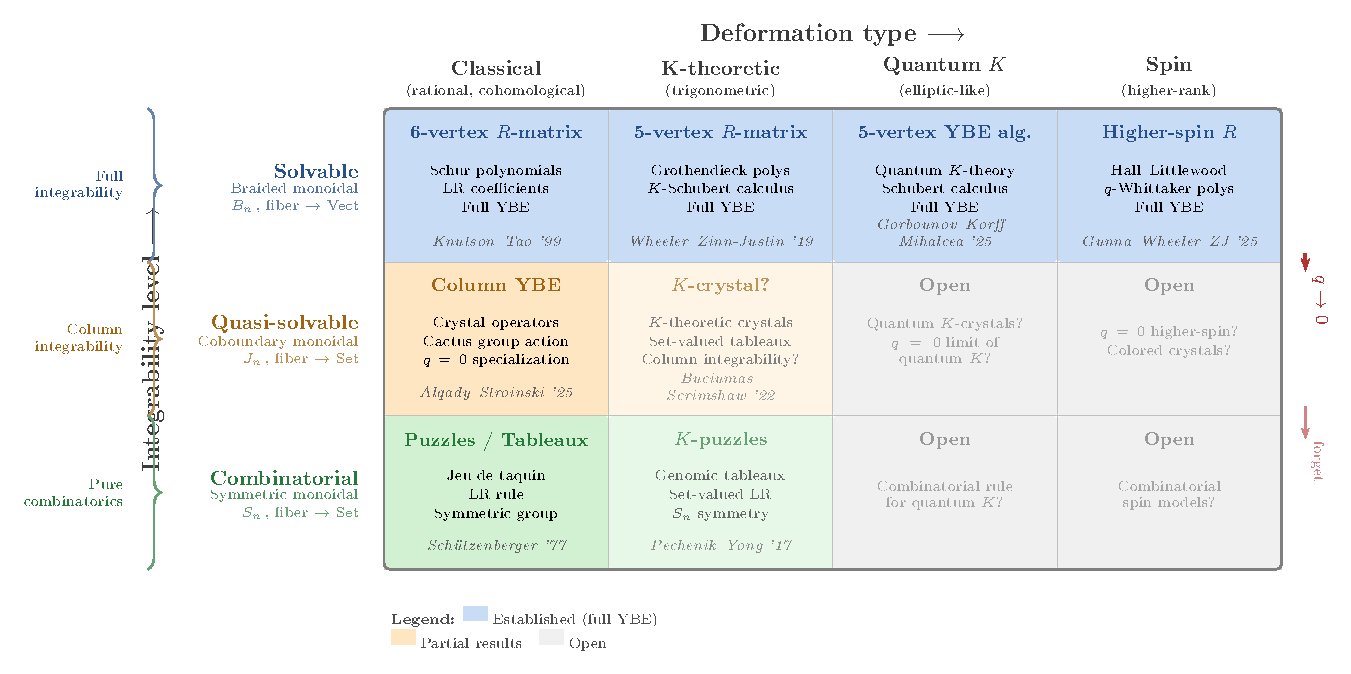
\includegraphics[width=\textwidth]{phase-diagram.pdf}
\caption{The categorical phase diagram.  The vertical axis parameterises
the integrability level (equivalently, the monoidal category type);
the horizontal axis parameterises the deformation type.  Filled cells
have established lattice models; lightly shaded cells have partial
results; empty cells are open.  The downward arrows indicate the
forgetful functors governed by the Hecke chain
$H_q \to H_0 \to \mathbb{C}[S_k]$.}
\label{fig:phase-diagram}
\end{figure}

\subsubsection*{A third dimension?}

The Tikhonov invariant $\kappa = (1-qp)/(1-p)$ suggests that the
phase diagram may have more structure than a flat grid.
The M\"obius formula~\eqref{eq:mobius} foliates the $(p,q)$ plane
into curves of constant $\kappa$: each curve represents a one-parameter
family of $(p,q)$ values producing the same asymptotic behaviour.  The
cactus locus --- the set of $(p,q)$ values where the cactus generator
emerges at $p = 1/2$ --- traces the line $\kappa = 2 - q$, a
constraint relating the interpolation and deformation parameters.

\begin{question}
Is the M\"obius action on $(p,q)$ related to the $\mathrm{PGL}(2)$
action on spectral parameters (Remark~\ref{rem:pgl2})?  If so, $\kappa$
would serve as a coordinate on a third axis --- the \emph{transition depth}
between integrability levels --- and the phase diagram would live on a surface
rather than a plane, with vertical transitions mediated by a continuous invariant.
One can test this by computing R-matrix eigenvalues and the Tikhonov invariant
$\kappa$ for small examples and checking whether they transform under the same
$\mathrm{PGL}(2)$.
\end{question}

\subsubsection*{What the diagram explains}

We close by returning to the question that opened the paper: why do so
many independent combinatorial models for LR coefficients exist?

The phase diagram provides an answer at two levels.  \emph{Horizontally},
models proliferate because the Yang-Baxter equation generates the
Yang-Baxter groupoid (Section~\ref{sec:groupoid-bn}): every R-matrix
move produces a new model computing the same coefficient.  The groupoid
is rich because the YBE has many solutions and many symmetries; the
bijections between models are morphisms, not miracles.
\emph{Vertically}, models proliferate because the categorical hierarchy
provides multiple projections of the same structure: the braided level
sees the spectral parameter, the coboundary level sees the multiplicity
bundle, and the symmetric level sees only the bare coefficient.  Each
level has its own characters, its own symmetry group, its own notion
of integrability --- and each level casts its own combinatorial
shadow.

The coefficients themselves --- $c^\nu_{\lambda,\mu}$, those
nonnegative integers governing the multiplication of Schur functions
--- sit at the intersection of all projections.  They are the invariant
that every level computes, every model records, and every forgetful
functor preserves.  The multiplicity of descriptions is not a defect
of the theory but a reflection of its depth: the same integers, seen
from above through a spectral parameter, from the middle through a
multiplicity bundle, and from below through a crystal basis, look
different at each level but agree on the count.  The phase diagram
is the map that says which view you are taking and what you have
chosen not to see.

%% Section 6: The Shuffle Algebra Substrate
%% To be \input{} into the main document.

\section{The Shuffle Algebra Substrate}
\label{sec:shuffle}

The three-level hierarchy of Section~\ref{sec:hierarchy} organises the
space of LR models vertically (by integrability level) and
horizontally (by deformation type).  But the hierarchy itself sits
inside a larger algebraic universe.  In this section we sketch the
contours of that universe: the \emph{shuffle algebra} framework, which
provides a single algebraic substrate from which all the integrable
vertex models of this paper can be derived.

\subsection{Feigin-Odesskii shuffle algebras}
\label{sec:shuffle-def}

Let $V$ be a finite-dimensional vector space and let
$\zeta(z) \in \mathbb{C}(z)$ be a rational function, called the
\emph{shuffle kernel}.  The \emph{Feigin-Odesskii shuffle
algebra}~\cite{feigin-odesskii} is defined on the direct sum
\[
  \mathcal{S}_\zeta \;=\; \bigoplus_{n \geq 0} \mathbb{C}(z_1, \ldots, z_n),
\]
with multiplication given by the \emph{shuffle product}: for
$f \in \mathbb{C}(z_1, \ldots, z_m)$ and
$g \in \mathbb{C}(z_1, \ldots, z_n)$,
\begin{equation}\label{eq:shuffle-product}
  (f \star g)(z_1, \ldots, z_{m+n})
  \;=\;
  \mathrm{Sym}\!\left[
    f(z_1, \ldots, z_m) \cdot g(z_{m+1}, \ldots, z_{m+n})
    \cdot \prod_{i=1}^{m} \prod_{j=m+1}^{m+n}
    \zeta\!\left(\frac{z_i}{z_j}\right)
  \right],
\end{equation}
where $\mathrm{Sym}$ denotes symmetrisation over all
$(m,n)$-shuffles of the variables $z_1, \ldots, z_{m+n}$.  The
shuffle kernel $\zeta$ controls the algebra: different choices of
$\zeta$ produce genuinely different algebraic structures.  At the
extreme $\zeta \equiv 1$, the shuffle product reduces to ordinary
symmetrisation and $\mathcal{S}_\zeta$ is the algebra of symmetric
rational functions.  Nontrivial kernels introduce interaction between
the two factors, and it is precisely this interaction that encodes the
Boltzmann weights of integrable lattice models.

\subsection{From shuffle algebras to vertex models}

The connection to our story was established by Garbali and
Gunna~\cite{garbali-gunna-2024}, who proved that the vertex models
computing symmetric function structure constants---including the
Schur, Grothendieck, and Hall-Littlewood models of
Section~\ref{sec:lattice}---can be realised as \emph{representations}
of appropriate shuffle algebras.  More precisely, the row operators of
the lattice model (the transfer matrices $T(u)$ of
Section~\ref{sec:lattice-transfer}) intertwine the shuffle product
with the composition of vertex weights: the algebraic identity
$T(u) \star T(v) = T(u) \circ T(v)$ (suitably interpreted) encodes
both the Yang-Baxter equation and the commutativity of transfer
matrices in a single stroke.

Garbali and Negut~\cite{garbali-negut-2025} extended this picture by
proving that the shuffle algebra $\mathcal{S}_\zeta$, for the kernel
$\zeta(z) = (z - 1)/(z - q)$ relevant to the Schur/Hall-Littlewood
family, is isomorphic to the positive part $U_q^+(\widehat{\mathfrak{gl}}_1)$
of the quantum toroidal algebra (equivalently, the positive half of
the Yangian $Y(\widehat{\mathfrak{gl}}_1)$ at the rational level).
This isomorphism is not merely formal: it identifies the shuffle
generators with specific combinations of Drinfeld currents, and under
this identification, the vertex model partition functions become
matrix elements of intertwining operators between Fock space modules.
The consequence is stark: \emph{all} the integrable lattice models
from Section~\ref{sec:lattice}---Schur, Grothendieck,
Hall-Littlewood, $q$-Whittaker---are manifestations of a single
algebraic structure, viewed through different representations.

\subsection{Connection to the Hecke algebra}

The shuffle algebra also makes contact with the Hecke transition
algebra of Section~\ref{sec:hierarchy}.  Kalmykov~\cite{kalmykov}
established explicit isomorphisms connecting three objects at the
rational level:
\begin{enumerate}
\item the Feigin-Odesskii shuffle algebra $\mathcal{S}_\zeta$;
\item the \emph{degenerate affine Hecke algebra} (dAHA)
  $H_n^{\mathrm{aff}}$, which extends the finite Hecke algebra $H_q(S_n)$
  by polynomial generators $x_1, \ldots, x_n$ satisfying the
  Bernstein-Lusztig relations; and
\item the Yangian $Y(\mathfrak{gl}_n)$.
\end{enumerate}
Since the finite Hecke algebra $H_q(S_n)$ embeds in the dAHA as the
subalgebra generated by the simple transpositions (without the
polynomial generators), the Hecke transition algebra from
Section~\ref{sec:hierarchy} sits inside the shuffle substrate as a
natural subalgebra.  The three-level hierarchy
$H_q \to H_0 \to \mathbb{C}[S_n]$ is a shadow of a deeper hierarchy
within the Yangian, where the specialisation $q \to 0$ corresponds to
a contraction of the quantum group to its classical limit.

\subsection{The emerging picture}

The shuffle algebra framework suggests a four-level depth hierarchy
for understanding why the LR coefficients admit so many combinatorial
models:

\begin{enumerate}
\item \textbf{Combinatorial bijections.}  At the surface, one has
  explicit maps between tableaux, puzzles, pipe dreams, and other
  models.  These bijections are typically proved by induction or
  sign-reversing involutions, and their existence appears miraculous.

\item \textbf{Yang-Baxter groupoid.}  One level down, the bijections
  are morphisms in the Yang-Baxter groupoid of Bump and
  Naprienko~\cite{bump-naprienko-2025}
  (Section~\ref{sec:groupoid-bn}).  Their existence follows from the
  Yang-Baxter equation: each R-matrix move preserves the partition
  function, so composing moves gives a canonical bijection.  The
  miracle is demystified but not fully explained---one still needs to
  know \emph{why} the R-matrix satisfies the YBE.

\item \textbf{Shuffle algebra.}  At the next level, the R-matrices
  are intertwining operators for representations of the shuffle
  algebra $\mathcal{S}_\zeta$.  The YBE is a consequence of the
  associativity of the shuffle product, and the multiplicity of
  lattice models reflects the multiplicity of representations.
  Different representations give different vertex weights, but the
  partition functions agree because the underlying algebra is the
  same.

\item \textbf{Geometric Satake.}  At the deepest level (which we do
  not develop here), the shuffle algebra is the cohomology of a
  moduli space of instantons, and the LR coefficients are intersection
  numbers on the affine Grassmannian.  The geometric Satake
  correspondence~\cite{mirkovic-vilonen-2007} provides the ultimate
  explanation: the structure constants of the representation ring are
  geometric invariants, and their positivity is a consequence of the
  decomposition theorem in perverse sheaves.
\end{enumerate}

\noindent
Each level subsumes the ones above it, offering a deeper explanation
for the same numerical coincidences.  The categorical phase diagram of
Section~\ref{sec:hierarchy} lives at levels~2 and~3: the vertical
axis (integrability level) is governed by the Hecke quotients of the
shuffle algebra, while the horizontal axis (deformation type) is
governed by the choice of shuffle kernel~$\zeta$.  The full picture---a
phase diagram sitting inside the representation theory of a shuffle
algebra, itself a shadow of geometric Satake---remains to be completed.
We turn to the open questions in the next section.

%% Section 7: Open Questions and Future Directions
%% To be \input{} into the main document.

\section{Open Questions and Future Directions}
\label{sec:open}

We organise the questions suggested by this paper into three tiers,
roughly ordered by accessibility: problems that could be attacked with
existing tools, problems that require new ideas, and problems that
call for significant new theory.


\subsection{Immediately tractable}

\begin{enumerate}[label=\textbf{Q\arabic*.}, ref=Q\arabic*, leftmargin=3em]

\item \label{q:horizontal}
\textbf{Complete the phase diagram horizontally.}
The categorical phase diagram of Section~\ref{sec:hierarchy} has
populated cells in every column of the solvable row (Schur,
Grothendieck, quantum $K$, Hall-Littlewood) and in the classical
column of the coboundary row (Demazure crystals).  The remaining
coboundary cells---K-theoretic, quantum K-theoretic, and spin models
at the quasi-solvable level---are open.  Yang's Demazure crystal
model~\cite{yang-2025} covers the classical coboundary column; the
K-theoretic and spin columns at this level remain to be constructed.
Concretely: which lattice models compute coboundary-level structure
constants for Grothendieck polynomials and Hall-Littlewood polynomials?
Do they exhibit the factored (column-level) YBE characteristic of
quasi-solvability?

\item \label{q:typeCD}
\textbf{Type C/D phase diagram.}
Everything in this paper concerns type~$A$---the general linear group
and its symmetric functions.  Azenhas, Feller, and
Torres~\cite{azenhas-feller-torres-2022} construct the symplectic
cactus group action on type~$C$ crystals, discovering additional
relations beyond those present in type~$A$.  What does the
integrability hierarchy look like for $\mathrm{Sp}_{2n}$?  The
quasi-solvable lattice models of Buciumas and
Scrimshaw~\cite{buciumas-scrimshaw} for types $B$, $C$, and $D$
provide the integrable side of the story; the categorical side---what
replaces the cactus group, whether the Hecke transition algebra
admits a type $C$ analogue---is largely unexplored.

\item \label{q:cactus-splitting}
\textbf{$J_n$ non-splitting for all~$n$.}
The cactus group $J_n$ fits into a short exact sequence
$1 \to PJ_n \to J_n \to S_n \to 1$,
where $PJ_n$ is the \emph{pure cactus group}.  For $n = 3$, we proved
by four independent methods (including the computation
$H^2(S_3, \mathbb{Z}^{\mathrm{sgn}}) \cong \mathbb{Z}/3\mathbb{Z}$)
that this sequence does not split.  Non-splitting is the algebraic
counterpart of the geometric fact that the real moduli space
$\overline{M}_{0,n+1}(\mathbb{R})$ is not a trivial $S_n$-bundle.

For $n \geq 4$, the pure cactus group is non-abelian, so the
classical group cohomology approach (which requires abelian
coefficients) does not directly apply.  The most promising route is
topological: Devyatov's presentation~\cite{devyatov-2015} of the
fundamental group of $\overline{M}_{0,n+1}(\mathbb{R})$ expresses the
pure cactus group in terms of explicit generators and relations.  A
careful analysis of these relations---perhaps combined with the
non-abelian cohomology $H^1(S_n, \mathrm{Out}(PJ_n))$---should settle
the non-splitting question for all~$n$.

\end{enumerate}


\subsection{Medium-term}

\begin{enumerate}[label=\textbf{Q\arabic*.}, ref=Q\arabic*, leftmargin=3em]
\setcounter{enumi}{3}

\item \label{q:spectral-parameter}
\textbf{$\kappa$ as spectral parameter.}
Tikhonov~\cite{tikhonov-2026} showed that the limiting permuton of a
random sorting network is governed by the invariant
$\kappa = (1 - qp)/(1-p)$, and that the M\"obius transformation
$p' = p(1-q)/(1-qp)$ relates the braided ($q > 0$) and coboundary
($q = 0$) regimes.  This transformation is an element of
$\mathrm{PGL}(2)$, acting on the probability parameter $p$ with the
Hecke parameter $q$ as coefficient.

The same group $\mathrm{PGL}(2)$ acts on the spectral parameter $u$
in the Yang-Baxter equation: the R-matrix $R(u)$ of a rational
model transforms under $u \mapsto (au + b)/(cu + d)$ by
conjugation.  Is Tikhonov's M\"obius transformation the \emph{same}
$\mathrm{PGL}(2)$ element that relates the spectral parameters of the
braided and coboundary R-matrices?  An affirmative answer would give a
quantitative, parameter-level avatar of the forgetful functor
$\mathrm{Braided} \to \mathrm{Coboundary}$ from
Section~\ref{sec:hierarchy}.

\item \label{q:cactus-yang}
\textbf{Cactus action on Yang's boundary conditions.}
Yang's Demazure crystal model~\cite{yang-2025} is parameterised by a
permutation $w \in S_r$, which enters as the boundary condition on the
right edge of the lattice.  The cactus group $J_r$ acts on Demazure
crystals via compositions of Sch\"utzenberger
involutions~\cite{henriques-kamnitzer-2006}.  Does the cactus action
on the crystal correspond to a permutation of Yang's boundary
conditions---that is, does the cactus generator $s_{[i,j]}$ send the
boundary condition $w$ to $w \cdot w_0^{[i,j]}$, where $w_0^{[i,j]}$
is the longest element of $S_{\{i, \ldots, j\}}$?  If so, the
coboundary commutor would have an explicit lattice-model
manifestation: it permutes the boundary data, and the resulting
bijection on configurations is the lattice-model avatar of the
Sch\"utzenberger involution.

\item \label{q:specialization-moduli}
\textbf{Specialization moduli.}
Fan, Guo, and Xiong~\cite{fan-guo-xiong} proved that KTW puzzles and
bumpless pipe dreams are not independent models but rather
\emph{specialisations} of a single lattice model: different choices of
boundary conditions and spectral parameters in one unified vertex model
recover both combinatorial objects.  What is the \emph{moduli space} of
all such specialisations?  Is it related to the space of factored
integrability conditions (the locus where $R_{\mathrm{row}}$ and
$R_{\mathrm{col}}$ independently satisfy the YBE)?  A complete
description of this moduli space would answer, in a precise sense,
the question ``how many essentially different combinatorial models for
the LR coefficients exist?''

\end{enumerate}


\subsection{Long-term}

\begin{enumerate}[label=\textbf{Q\arabic*.}, ref=Q\arabic*, leftmargin=3em]
\setcounter{enumi}{6}

\item \label{q:shuffle-full}
\textbf{Shuffle algebra for the full phase diagram.}
The Garbali-Negut isomorphism~\cite{garbali-negut-2025} connects
shuffle algebras to Yangians at the rational level, which governs the
classical (cohomological) column of the phase diagram.  Does this
isomorphism extend to the trigonometric level (K-theoretic column,
where the relevant quantum group is the quantum affine algebra
$U_q(\widehat{\mathfrak{sl}}_n)$) and the elliptic level (where the
quantum group is Felder's elliptic quantum
group~\cite{felder-1995})?  The Shibukawa-Ueno
hierarchy~\cite{shibukawa-ueno}---elliptic, trigonometric,
rational---classifies R-matrices by the function field in which they
live, and is \emph{orthogonal} to the braided/coboundary/symmetric
hierarchy of Section~\ref{sec:hierarchy}.  The intersection of these
two hierarchies would give a three-dimensional phase diagram: one axis
for deformation type, one for integrability level, and one for the
analytic class of the R-matrix.

\item \label{q:tqft}
\textbf{TQFT for puzzle bundles.}
The failure of the Zinn-Justin tetrahedron equation at the
quasi-solvable level (Section~\ref{sec:groupoid-hierarchy}) defines a
curvature 2-form on the ``puzzle bundle'' over the higher Bruhat order
$B(n,2)$.  This curvature measures the obstruction to promoting
column-level integrability to full vertex-level integrability, and its
holonomy around closed loops encodes the non-abelian structure of the
pure cactus group.  Is there a topological quantum field theory whose
partition function computes LR coefficients, with the curvature
encoding the quasi-solvable level?  Such a TQFT would provide a
geometric home for the categorical phase diagram: the braided level
would correspond to a flat connection (zero curvature, trivial
holonomy), the coboundary level to a curved connection with discrete
holonomy, and the symmetric level to the trivial bundle.

\item \label{q:kpz}
\textbf{KPZ universality for Schubert calculus.}
Morales, Panova, Petrov, and
Yeliussizov~\cite{morales-panova-petrov-yeliussizov} connect pipe
dreams to the totally asymmetric simple exclusion process (TASEP) and
Tracy-Widom distributions, placing classical Schubert calculus in the
KPZ universality class.  Does this connection extend to K-theoretic or
quantum K-theoretic Schubert calculus?  The K-theoretic structure
constants are \emph{signed}, which complicates the probabilistic
interpretation, but Tikhonov's permuton results~\cite{tikhonov-2026}
suggest that the probabilistic side is tractable whenever the Hecke
parameter $q$ is real.  A KPZ universality theorem for Grothendieck
polynomials would link the algebraic geometry of flag varieties to the
statistical mechanics of interface growth---two subjects that have
developed largely in parallel.

\end{enumerate}

\bigskip

\noindent
\textbf{Coda.}\enspace
The central message of this paper is that the multiplicity of
combinatorial models for LR coefficients is not a historical accident
but a structural inevitability.  The models proliferate because they
are representations of a rich algebraic object---the shuffle algebra
and its quotients---organised by the integrability hierarchy into
levels of increasing symmetry.  Each level forgets something precise
(a spectral parameter, a multiplicity bundle), and each forgetting
produces a simpler but still faithful encoding of the same
nonnegative integers.  Understanding this structure does more than
explain existing combinatorics: it predicts where new models should
live (the open cells of the phase diagram), identifies the invariants
that distinguish them (the Hecke parameter $q$, the shuffle
kernel~$\zeta$), and points toward deeper explanations (geometric
Satake, TQFT, KPZ universality) that may one day subsume the entire
picture.

The LR coefficients, those modest nonnegative integers governing the
multiplication of Schur functions, have turned out to be a window onto
a remarkably deep landscape.  We have tried to draw a map of what we
can see.  The territory beyond the map---the open cells, the
conjectural connections, the questions we do not yet know how to
ask---is, we suspect, richer still.


%%% Acknowledgements %%%
\section*{Acknowledgements}
% TODO: Add acknowledgements.

%%% Bibliography %%%
\begin{thebibliography}{99}

\bibitem{azenhas-feller-torres-2022}
O.~Azenhas, P.~L.~Feller, and J.~Torres,
\emph{Symplectic cacti, virtualization, and Berenstein--Zelevinsky data},
J. Comb.\ Algebra, to appear (2026).

\bibitem{baxter-1982}
R.~J.~Baxter,
\emph{Exactly Solved Models in Statistical Mechanics},
Academic Press, London, 1982.

\bibitem{borodin-wheeler-2018}
A.~Borodin and M.~Wheeler,
\emph{Coloured stochastic vertex models and their spectral theory},
arXiv:1808.01866 (2018).

\bibitem{brubaker-bump-buciumas-gustafsson-2021}
B.~Brubaker, D.~Bump, V.~Buciumas, and H.~P.~A.~Gustafsson,
\emph{Colored five-vertex models and Demazure atoms},
J. Combin.\ Theory Ser.~A \textbf{178} (2021), 105354.

\bibitem{brubaker-bump-hardt-spink}
B.~Brubaker, D.~Bump, A.~Hardt, and H.~Spink,
\emph{Kazhdan--Lusztig theory and the Yang--Baxter equation},
arXiv preprint (2024).

\bibitem{buciumas-scrimshaw}
V.~Buciumas and T.~Scrimshaw,
\emph{Quasi-solvable lattice models for $\mathrm{Sp}_{2n}$ and $\mathrm{SO}_{2n+1}$ Demazure atoms and characters},
arXiv:2201.01026 (2022).

\bibitem{bump-naprienko-2025}
D.~Bump and S.~Naprienko,
\emph{The Yang--Baxter equation and Schur functions},
arXiv preprint (2025).

\bibitem{devyatov-2015}
R.~Devyatov,
\emph{On subgroups of the pure cactus group},
arXiv:1507.04699 (2015).

\bibitem{fan-guo-xiong}
N.~Fan, P.~Guo, and R.~Xiong,
\emph{Bumpless pipe dreams meet puzzles},
arXiv preprint (2024).

\bibitem{fulton-1997}
W.~Fulton,
\emph{Young Tableaux: With Applications to Representation Theory and Geometry},
London Math.\ Soc.\ Student Texts \textbf{35}, Cambridge Univ.\ Press, 1997.

\bibitem{gaetz-gao-2024}
C.~Gaetz and Y.~Gao,
\emph{Integrable triangle-accessible lattice models},
arXiv preprint (2024).

\bibitem{galashin-2020}
P.~Galashin,
\emph{Symmetries of stochastic colored vertex models},
Ann.\ Probab.\ \textbf{49} (2021), no.~5, 2175--2219.

\bibitem{garbali-gunna-2024}
A.~Garbali and J.~Gunna,
\emph{Shuffle algebras and lattice paths},
arXiv preprint (2024).

\bibitem{garbali-negut-2025}
A.~Garbali and A.~Negut,
\emph{Shuffle algebras and Yangians},
arXiv preprint (2025).

\bibitem{gorbounov-korff-mihalcea-2025}
V.~Gorbounov, C.~Korff, and L.~Mihalcea,
\emph{Quantum $K$-theory and the Yang--Baxter equation},
arXiv preprint (2025).

\bibitem{gunna-wheeler-zj-2025}
J.~Gunna, M.~Wheeler, and P.~Zinn-Justin,
\emph{Spin Hall--Littlewood polynomials and vertex models},
arXiv preprint (2025).

\bibitem{henriques-kamnitzer-2006}
A.~Henriques and J.~Kamnitzer,
\emph{Crystals and coboundary categories},
Duke Math.~J.\ \textbf{132} (2006), no.~2, 191--216.

\bibitem{jimbo-1986}
M.~Jimbo,
\emph{A $q$-analogue of $U(\mathfrak{gl}(N+1))$, Hecke algebra,
and the Yang--Baxter equation},
Lett.\ Math.\ Phys.\ \textbf{11} (1986), no.~3, 247--252.

\bibitem{kalmykov}
A.~Kalmykov,
\emph{Shuffle algebra, degenerate affine Hecke algebra, and Yangian},
preprint.

\bibitem{kamnitzer-tingley-2007}
J.~Kamnitzer and P.~Tingley,
\emph{The crystal commutor and Drinfeld's unitarized $R$-matrix},
J.~Algebraic Combin.\ \textbf{29} (2009), no.~3, 315--335.

\bibitem{kashiwara-1990}
M.~Kashiwara,
\emph{Crystallizing the $q$-analogue of universal enveloping algebras},
Comm.\ Math.\ Phys.\ \textbf{133} (1990), no.~2, 249--260.

\bibitem{knutson-tao-1999}
A.~Knutson and T.~Tao,
\emph{The honeycomb model of $\mathrm{GL}_n(\mathbb{C})$ tensor products~I:
Proof of the saturation conjecture},
J.~Amer.\ Math.\ Soc.\ \textbf{12} (1999), no.~4, 1055--1090.

\bibitem{knutson-tao-woodward-2004}
A.~Knutson, T.~Tao, and C.~Woodward,
\emph{The honeycomb and saturation conjectures},
J.~Amer.\ Math.\ Soc.\ \textbf{17} (2004), no.~1, 19--48.

\bibitem{macdonald-1995}
I.~G.~Macdonald,
\emph{Symmetric Functions and Hall Polynomials},
2nd ed., Oxford Math.\ Monographs, Oxford Univ.\ Press, 1995.

\bibitem{morales-panova-petrov-yeliussizov}
A.~H.~Morales, G.~Panova, L.~Petrov, and D.~Yeliussizov,
\emph{Grothendieck shenanigans},
arXiv preprint (2024).

\bibitem{norton-1979}
P.~N.~Norton,
\emph{$0$-Hecke algebras},
J.~Austral.\ Math.\ Soc.\ Ser.~A \textbf{27} (1979), no.~3, 337--357.

\bibitem{purbhoo-2007}
K.~Purbhoo,
\emph{Puzzles, tableaux, and mosaics},
J.~Algebraic Combin.\ \textbf{28} (2008), no.~4, 461--480.

\bibitem{savage-2020}
A.~Savage,
\emph{Crystals, coboundary categories, and the commutor},
lecture notes (2020).

\bibitem{stanley-1999}
R.~P.~Stanley,
\emph{Enumerative Combinatorics}, vol.~2,
Cambridge Studies in Adv.\ Math.\ \textbf{62}, Cambridge Univ.\ Press, 1999.

\bibitem{tikhonov-2026}
K.~Tikhonov,
\emph{Random permutations from $q$-Demazure products},
arXiv:2604.06532 (2026).

\bibitem{wheeler-zinn-justin-2016}
M.~Wheeler and P.~Zinn-Justin,
\emph{Littlewood--Richardson coefficients for Grothendieck polynomials
from integrability},
J.~Reine Angew.\ Math.\ \textbf{757} (2019), 159--195.

\bibitem{yang-2025}
J.~Yang,
\emph{Closed colored lattice models and Demazure crystals},
arXiv:2512.05479 (2025).

\end{thebibliography}

\end{document}
